\ifgerman{\chapter{Evaluierung}}{\chapter{Evaluation}}
\label{evaluation}

In this section, we will briefly discuss our evaluation methodology, which includes the criteria to measure whether the goals of this work were accomplished or not, as well as the structure and results of our testing.

\section{Objective and measurements}

To rate the effectiveness of the proposed methods we need a clearly stated and verifiable goal, including criteria to compare them against other techniques. This is easiest using the same scenario already used to describe the functioning of our methods: suppose we have a classifier, trained by an active learner using $k$ training instances. Then the objective of our methods is to estimate the classification loss of said classifier on data not yet seen, but from the same distribution as the training instances. Then, the bias and error of the estimation is to be compared against established estimators. The exact methods and the competition will be presented in the next section.

To compare the techniques, we utilize the error measures used in \cite{FigueroaEtal2012}, \textit{root mean squared error} (RMSE) and \textit{mean error} (ME), defined as
\begin{equation}
RMSE = \frac{1}{n} \sum_{i=1}^{n} \left(y_n - y_n^{'}\right)^2
\end{equation}
and
\begin{equation}
ME = \frac{1}{n} \sum_{i=1}^{n} y - y_n^{'},
\end{equation}
where $y_i$ is the reference accuracy, $y_i^{'}$ the estimate of a method and $n$ the number of test runs. $RMSE$ will tell us how wide the error is spread, while the raw mean error gives an estimate of the bias each technique carries.

Depending on the method in question, we may have additional measures for comparison. As a by-product of the multiple curves fit when using path sub-sampling, the resulting estimates can be seen as a sample of a distribution. In turn, we can estimate that distribution by estimating the mean and the variance of the sample. Luckily, the choice of the distribution model to assume is fairly simple; most models are not suitable anyway, as they are defined on $\mathbb{R}$. Our estimates, however, are limited to $[0,1]$. Thus, only few distributions come to mind, one of which is the beta distribution, also being used for similar purposes by \cite{KremplEtAl2014}. It is dependent by two parameters, $p, q \in \mathbb{R}_{\le 0}$, with a density function defined as \cite{GuptaEtAl2004}
\begin{equation}
f_{p, q}(x) = \frac{x^{p-1}(1-x)^{q-1}}{\int_{0}^{1} u^{p-1}(1-u)^{q-1}}.
\end{equation}
The parameters are computable from mean and variance via
\begin{equation}
\begin{split}
E[X] &= \frac{p}{p+q} \\
var[X] &= \frac{p*q}{(p+q)^2(p+q+1)}
\end{split}
\end{equation}
Having the estimated distribution, we can then compute the difference between it and the "true" distribution via the \textit{Kullback-Leibler divergence} (KLD):
\begin{equation}
KLD(P:Q) = \int_{}^{} p(x) \cdot log\left(\frac{p(x)}{q(x)}\right) d\lambda (x),
\end{equation}
with $p(x)$ and $q(x)$ are the density functions of their respective distribution \cite{KullbackEtAl1951}. The KL divergence is an information-theoretical measure intended to compare two probability distributions. If the two are equal almost everywhere, the KLD will be zero, otherwise positive. Importantly, it is neither symmetrical nor does it satisfy the triangular inequality, thus the choice of distribution assignment is meaningful and should be equal for all tested methods (i.e. the distribution P is always the reference distribution) \cite{Joyce2011}.

Although not the main focus, we will also keep an eye on the computation time needed for each method, mostly because of the exponential complexity of our proposed methods.

\section{Method selection}

The methods we described in section \ref{methods} mostly conform to a three-step process: First, some sort of sub-sampling is performed (whether this actually reduces the amount of subsets is irrelevant). Then, the performance for the selected subsets is estimated and grouped. Last, the function of choice is fit on the groups and the final performance estimate obtained by evaluating and then averaging the functions at the point $f(k)$. Including the possibility of using fitting improvements like weighting and the no-information rate as well as different function models, we get a lot of combinations available. Unfortunately, we cannot test all of them as it is quite time consuming, which necessitates the selection of some combinations.

Of course there are some intuitive limitations to what can be combined. When using all or a capped amount of subsets, applying some kind of path-like grouping seems much weirder than using averaging. Likewise, when path sub-sampling has been chosen, the intuitive option is to fit individual curves instead of only one with prior averaging. Also, some pre-screening suggested that the usage of the no-information rate as 0th data point is not as effective as hoped. Causes seem to be both high variance, leading to worsened fitting with low amounts of sub-samples, as well as its expendability for larger sub-sample sizes, which come naturally with larger training set sizes.

As a result of this, we designed tests for four different methods: path sub-sampling with as well as without superset restriction and one curve per path, which will be abbreviated as \textit{pathNormal} and \textit{pathSuper}, and capped sub-sampling with averaging and one curve fit, \textit{averaged}. While the estimation technique for the two path-based methods will be exclusively cross-validation, we elected \textit{averaging} to also be tested with .632 bootstrapping to assess whether it has any impact on the quality of the methods. Additionally, we will evaluate each of them using both weighted and unweighted fitting, with the former being designated by a trailing \textit{W}. And although the pre-screening made the usage of the no-information rate questionable, not testing it at all would be a waste. Thus, \textit{pathSuper} also does participate in a modified version with a 0th data point for each path/curve, named \textit{pathSuperNI}.

\section{Test environment}

\subsection{Function models}

As kind of belonging to the estimation methods but not really, we separated the function model used for fitting from the method description. Since it does not affect their modus operandi, the choice of a model is, similar to the active learner and classifier, part of the test parameters. We already briefly touched on this subject in section \ref{methods} and mentioned the exponential law with three parameters as well as a custom sigmoid function with fairly descriptive parameters. As overfitting is a known problem for classification and regression \cite{Dietterich1995}, we also chose to test with a linear model, which also did decent in experiments on learning curve fitting \cite{FigueroaEtal2012}. Concluding, we have the following three function models for use:
\begin{subequations}
	\begin{align}
	f_{exp}(x) &= a + b \cdot e^{c \cdot x} \\
	f_{sig}(x) &= y_0 + 2 \cdot (y_0 - S) \cdot \left( \frac{1}{1+e^{m \cdot x}} - 0.5 \right) \\
	f_{lin}(x) &= m \cdot x + b
	\end{align}
\end{subequations}

Since a linear curve cannot accommodate for the bent shape of a typical learning curve we will only use the estimates corresponding to the subset sizes $k-4,...,k-1$ for its fitting, rather trying to predict the learning curves gradient and using the linear function as a tangent.

As the first two functions, exp and sig, are not linearizable, we have to use the Levenberg-Marquardt algorithm, which, amongst others, requires the specification of initial parameters. Also, as we do have a preconceived image of a learning curve as monotone rising and limited to the interval $[0, 1]$, providing constraints to fulfill these requirements seems proper. This is trivial for the sigmoid function, as it was specifically designed to allow this kind of modification: $y_0$ and $S$, as representations of the y-intercept and the function's asymptote, are limited to $[0,1]$ with $y_0 \leq S$, and $m$ has to be in $\mathbb{R}_{\geq 0}$. For the other functions it is not as easy to find suitable bounds: while both have parameters directly affecting the y-intercept and slope, their asymptote for $x \mapsto \inf$ is either affected by two parameters or is not a constant (linear). Both would require polynomial equality constraints, which were not taken into account for this work. Thus, it is good to keep in mind that these functions might violate the learning curve constraints.

\subsection{Active learner}

Although nothing in this work is directly dependent of it, the active learner (AL) used to select the instances is a core part of the evaluation. Not only because the whole sub-sampling is based on the assumption of an active learning process, but also due to the effect \textit{different} ALs have on the learning process: while a randomly sampling AL slowly but steadily gathers instances from everywhere in the feature space with equal probability, others put more emphasis on certain instances that may improve the classifier's performance more than others. One of the other ALs is \textit{uncertainty sampling}, which was already introduced in \ref{background}. Here, the data is assumed to be divided by a decision boundary, separating instances of different classes \cite{ZhuEtAl2008}. In case of an ideal separation, it will improve a classifier's accuracy quicker, i.e. it takes less purchased instances to reach a certain accuracy level. However, not all data has a clear decision boundary; noise and more than two groupings of instances sharing the same class make life difficult for uncertainty sampling.

\textit{Probabilistic active learning} (PAL) takes a different approach. It takes a look at each available instance's surroundings and computes the density of unlabeled as well as the amount of already purchased instances. The latter combined with the portion of instances sharing their class label with the original instance is denoted as \textit{label statistics}. Using this, assuming the instance's class label and the overall probability of this class in its neighbourhood was to be known, an optimal selection with regard to the classifier's performance could be made. But since those two quantities are generally unknown, PAL considers them as random variables. This enables the computation of an expected or probabilistic performance gain for each unlabeled instance. When weighted with the instance density in its neighbourhood, it allows an statistically optimal selection for the performance.

\begin{figure}[h]
	\centering
	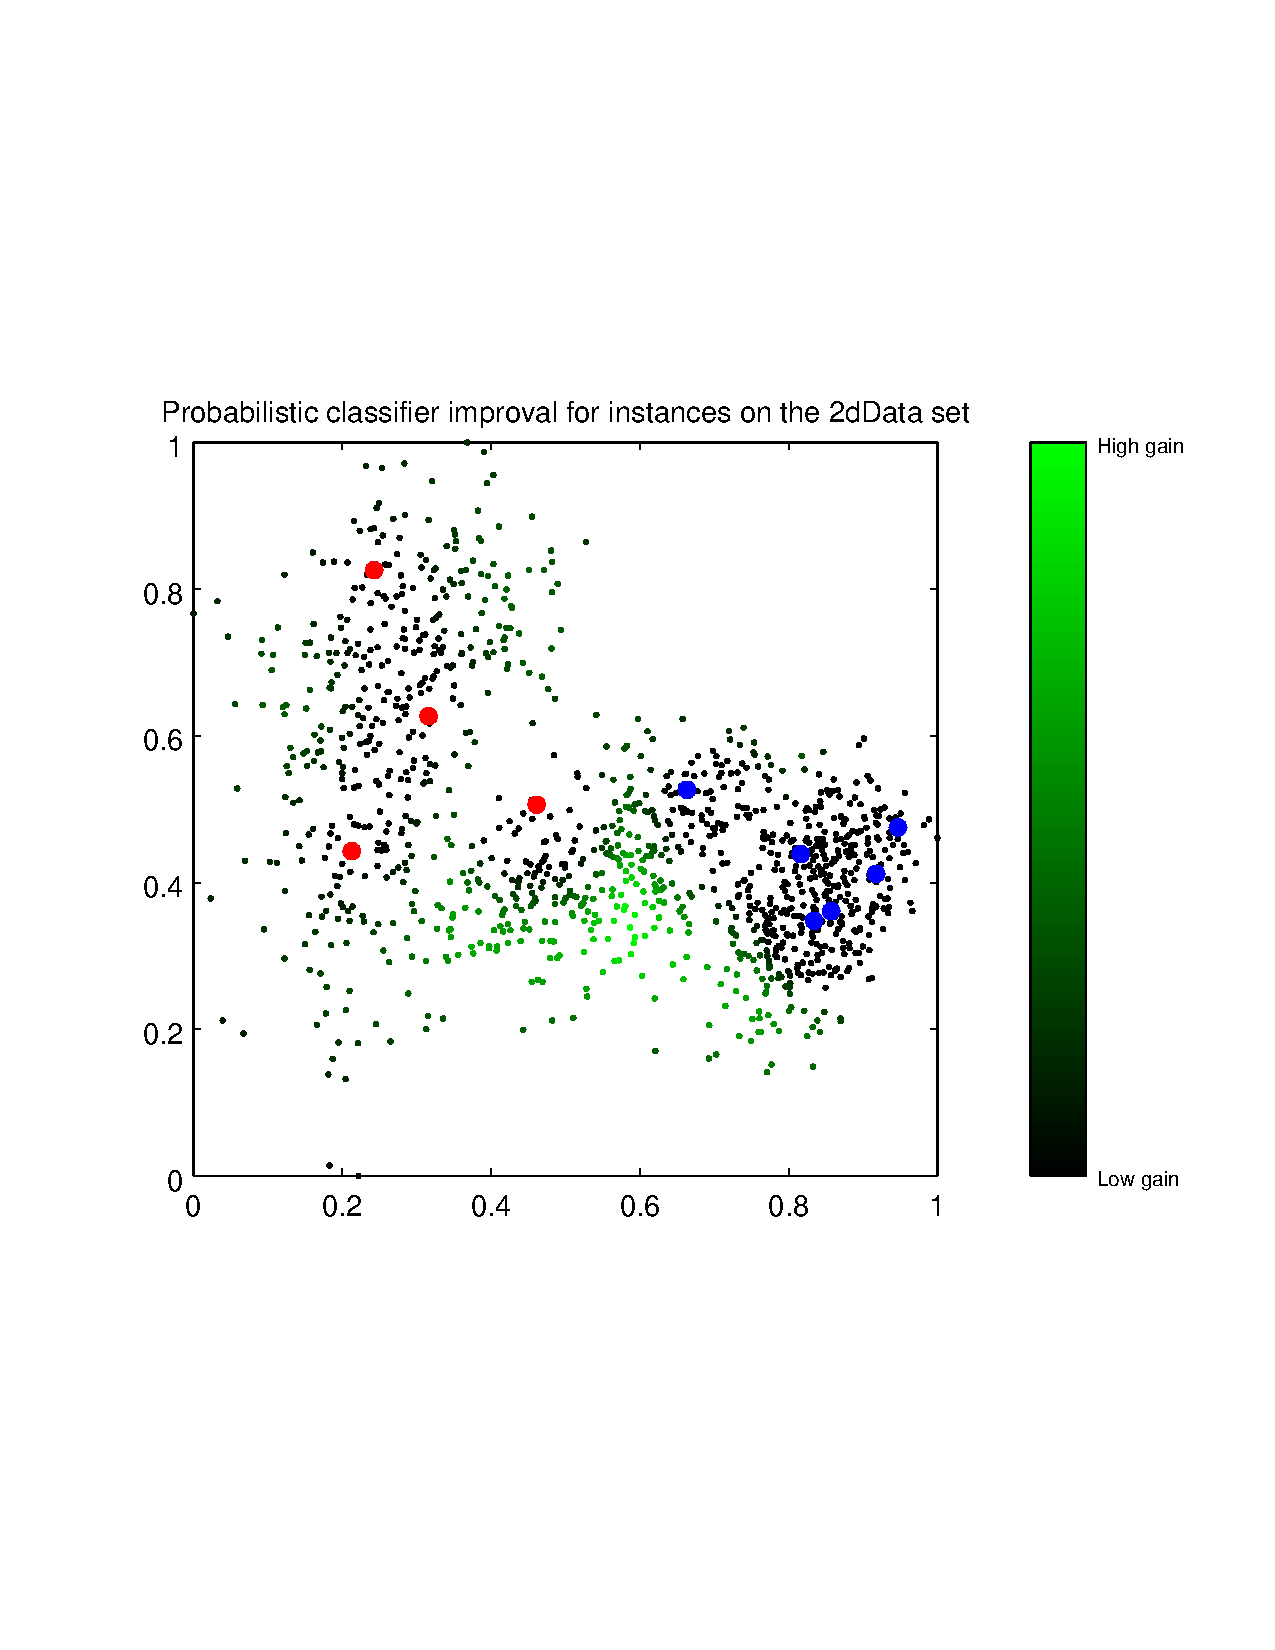
\includegraphics[trim = 0cm 6cm 0cm 5cm, clip = true, width = 0.8\textwidth]{PALIllustration}
	\caption{PAL illustration showing the weighted probabilistic gain (normed on $[0, 1]$). Since all labeled instances are grouped by their class label, the gain is higher for near the lower label-density group}
	\label{fig:PALIllustration}
\end{figure}

PAL makes some assumptions, one of which is that the class probability for a neighbourhood can be modeled as a beta distribution. In the original paper, the density computation was also performed with a modified version of kernel density estimation; more about this in \ref{evaluation:classifier}. However, since we use a different estimator for uncertainty sampling, this may hinder the comparability. Thus, instead of the originally intended estimator, we use our classifier for both active learners.

\subsection{Classifier}
\label{evaluation:classifier}
The choice of an adequate classifier is mostly limited by the active learners and the datasets used in the evaluation. From the dataset side, it has to be able to accept continuous features. The output of class assignment probability is necessitated by PAL and uncertainty sampling. Also, as PAL requires some sort of density estimation and to keep the comparability of both ALs up, a classifier making use of kernel density estimation (KDE) would be nice. Considering this, we selected the Parzen window classifier. It is a non-parametric classifier directly build on KDE. Here, we assume that the data is distributed according to some probability distribution; a good assumption is the normal distribution. Then, the kernel $K$, which in our case is the probability density function (but it does not have to be), is approximated at the point we want to know using the following formula:
\begin{equation}
\label{equ:uniKDE}
\hat{f}_h(x) = \frac{1}{nh} \sum_{i=1}^{n} K(\frac{x-x_n}{h})
\end{equation}
$x$ is the point for which we want to know the density, $x_n$ are the already known points and $h$ is the so-called bandwidth, a smoothing factor for the kernel \cite{SheatherEtAl1991}. It has to be estimated, which is usually done by applying a function called \textit{Silverman's rule of thumb}, which is dependent on $n$, the dimensionality of the data, its estimated standard deviation and some statistical properties of the kernel largely irrelevant to this work. If the data in question is multivariate, \eqref{equ:uniKDE} has to be a bit modified; $K$ is then usually the product of the kernel for each dimension, same goes for the bandwidth \cite{Silverman1986}.

\begin{figure}[h]
	\centering
	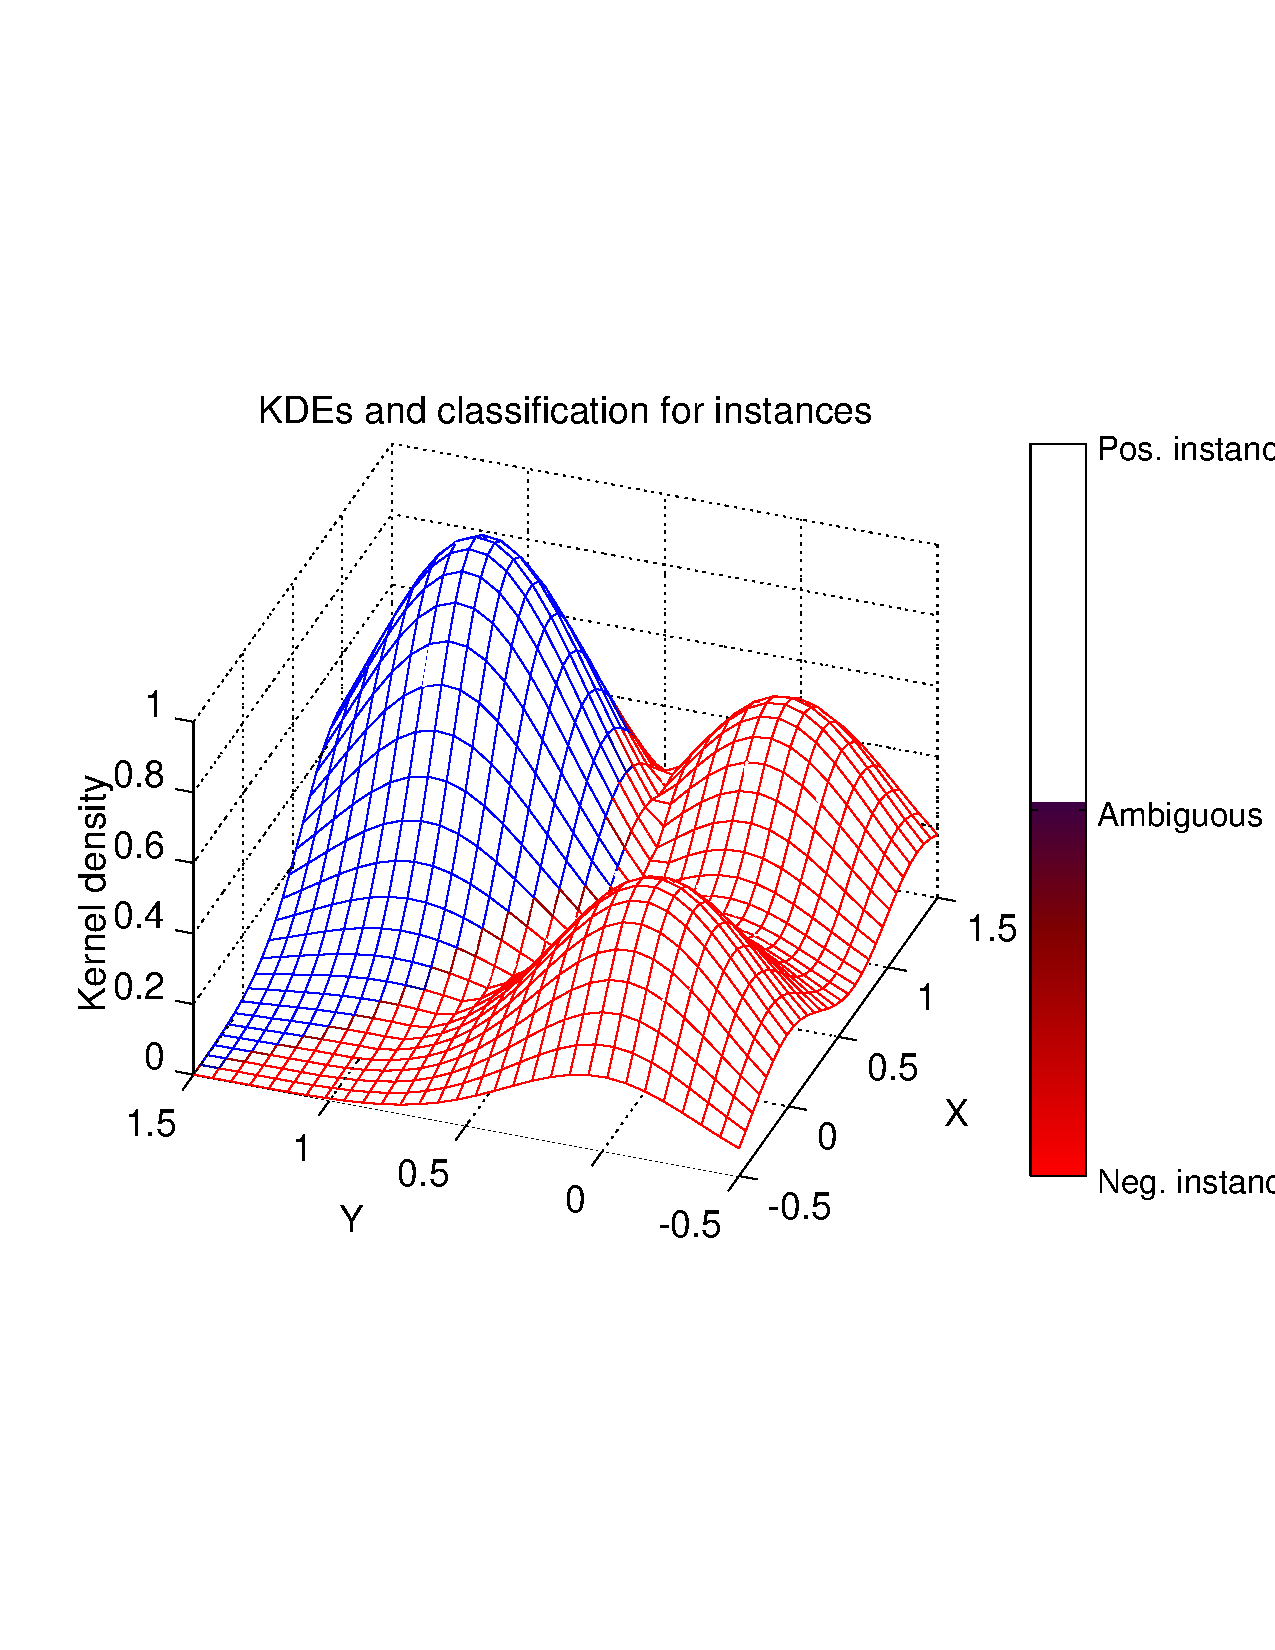
\includegraphics[trim = 0cm 6cm 0cm 5cm, clip = true, width = 0.8\textwidth]{KDE3inst}
	\caption{The estimated kernel density for a grid with one positive and two negative instance; lower Z value indicates lower certainty for the class assignment}
	\label{fig:KDE3inst}
\end{figure}

The Parzen window classifier estimates the densities of an instance to be labeled for each class label, each time using only the instances with the same label as $x_n$. Then, they are multiplied with the prior class probabilities, i.e. the share each class label has among the labeled instances. Normalization then results in the wanted (estimated) class probabilities, with the largest probability dictating the resulting class \cite{ArchambeauEtAl2006}.

\subsection{Datasets}

The selection of the datasets has to take some considerations into account. Firstly, the datasets should both be realistic and cover most uses; a method that does well on specifically designed test sets but fails in the real world is only interesting as a proof-of-concept. Secondly, PAL was only defined for dichotomous data. Although an extension on multiple-class problems should be possible, we did not want to tamper with the formulas and instead restrict the datasets to binary-class problems.

Considering these constraints we chose the following datasets:

\begin{itemize}
	\item \textbf{checke1}: This artificial dataset was used in \cite{Chapelle2005} to examine active learning with Parzen window classifiers and contains 400 instances with two features. It has the form of a 4x4 checkerboard, with only every second field containing instances. There is no overlapping of class labels, i.e. the instances can be perfectly separated by class label using decision boundaries. This set may be problematic for uncertainty sampling as it will select instances at its decision boundary, while the set requires \textit{multiple} decision boundaries. Thus, it likely will not label instances from the other fields until it runs out of close ones. Both random sampling and PAL should not have this problem; the former does not care about any structure anyway, while the latter actively explores the "uncharted" instances.
	\item \textbf{2dData}: Also an artificial, 2-dimensional dataset, it was used in the original PAL paper \cite{KremplEtAl2014}. The 1200 instances are grouped into two clusters of roughly ellipsoid shape, but cannot be perfectly separated as they slightly overlap, making it seem more realistic (real-world datasets tend to have some noisy data). None of the active learners should have inherent problems with this set.
	\item \textbf{seeds}: A real-world dataset used in \cite{CharytanowiczEtAl2010}. It has seven features which describe different properties of wheat, classifying it into three varieties: Rosa, Kama and Canadian with 70 instances each. To comply with the constraints set earlier, the varieties Kama and Canadian were merged into one class. As it is 7-dimensional, obtaining a visual is difficult; thus we used "t-Distributed Stochastic Neighbor Embedding (t-SNE)", a method for dimensionality reduction of high-dimensional data \cite{vanDerMaaten2008} to project it into $\mathbb{R}^2$ by using Gauss kernels to keep neighboring instances together. Similar to \textit{2dData}, two clusters seem to be present, each containing instances sharing the same class label, albeit a small overlap exists. Due to the similarity, no problems regarding the active learners are to be expected.
	\item \textbf{abalone}: A real-world dataset using eight predictors associated with predict the age of abalones. Originally, the number of rings (and thus ages) of a specimen were predicted. To create a binary set, all ages below 10 form one class, while the rest forms the other. The set was obtained in the study \cite{NashEtAl1994}. As the original set contained 4177 instances, it had to be reduced to remain a viable option, considering the finite amount of time available for testing. Thus, the number of instances was reduced to 1800, keeping the class ratio intact. The visualization indicates the presence of four separate clusters with partially mixed class labels. While this may hint at problems with uncertainty sampling, the study itself suggests that the predictors are not sufficient for classification, leading to high error rates even with large training sets.
\end{itemize}

\begin{figure}[h]
	\centering
	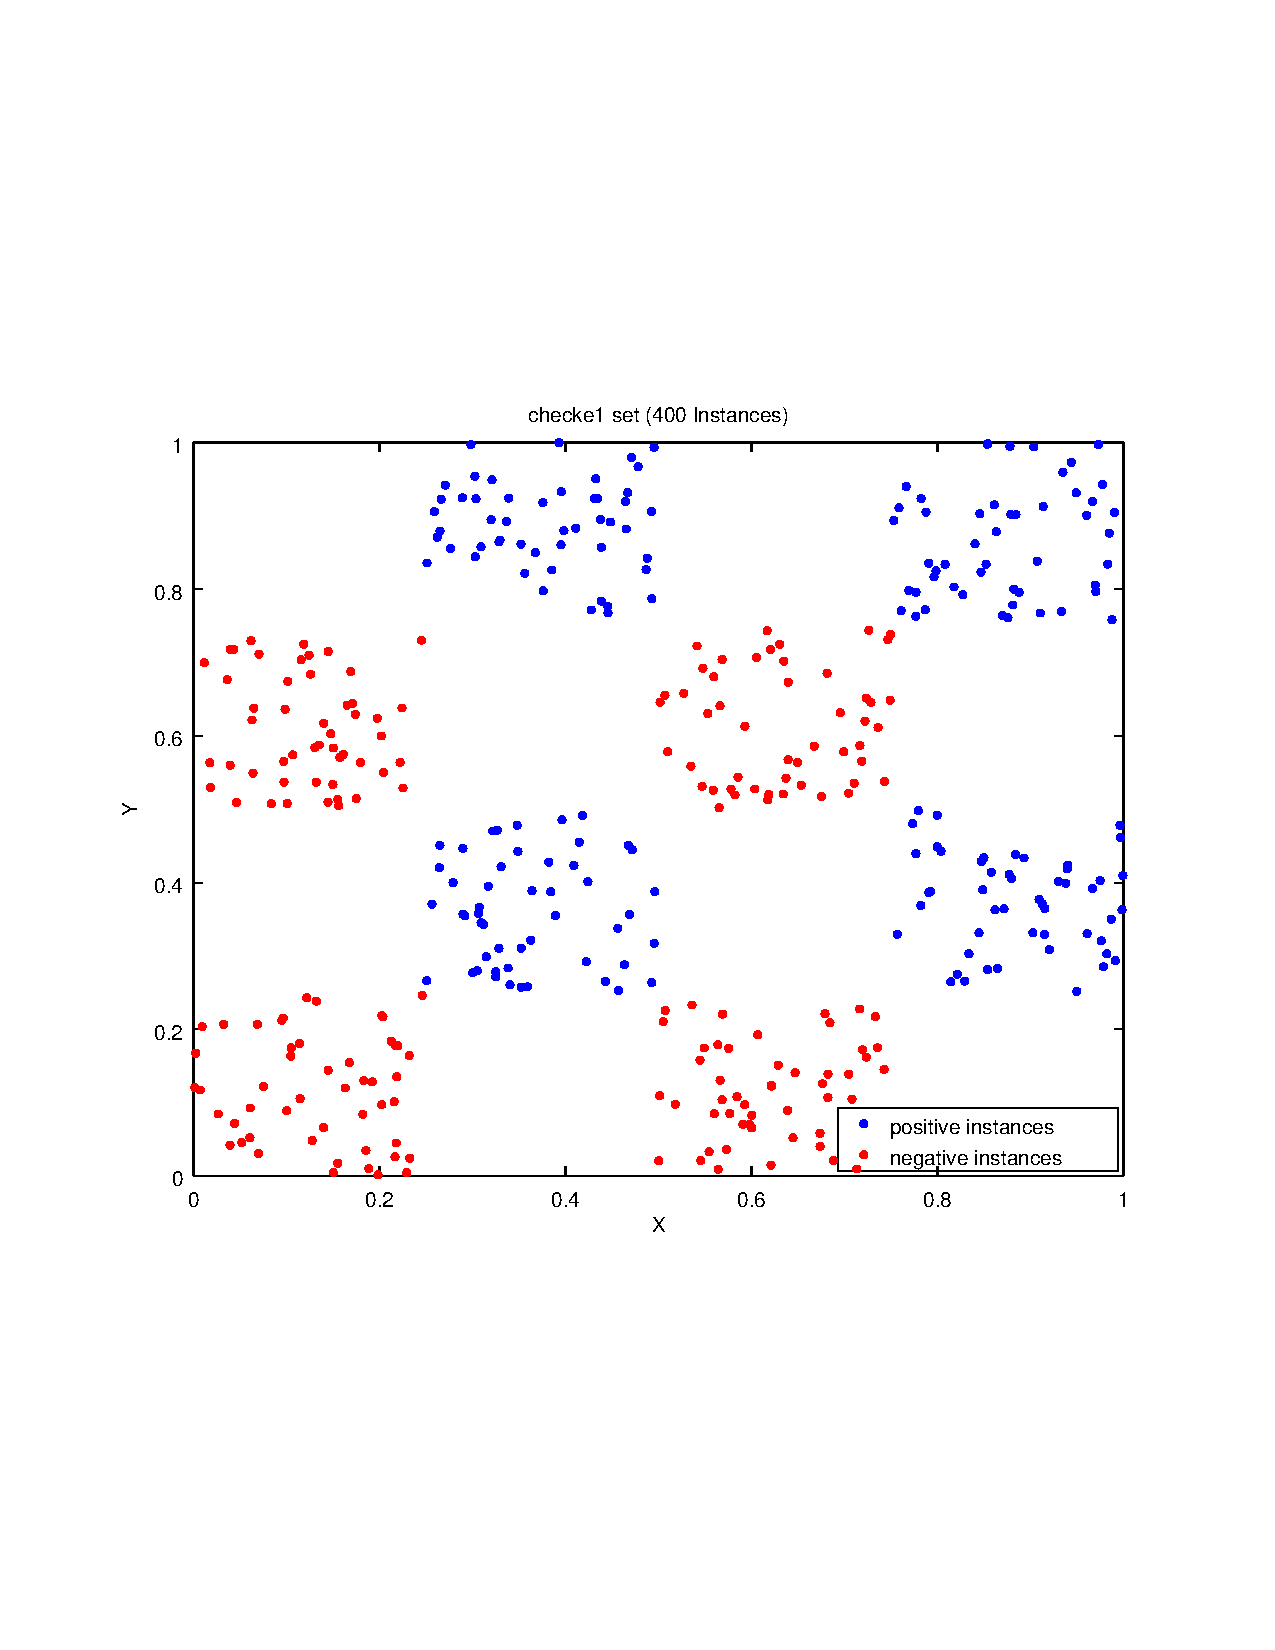
\includegraphics[trim = 0cm 6cm 0cm 5cm, clip = true, width = 0.45\textwidth]{checke1Illustration}
	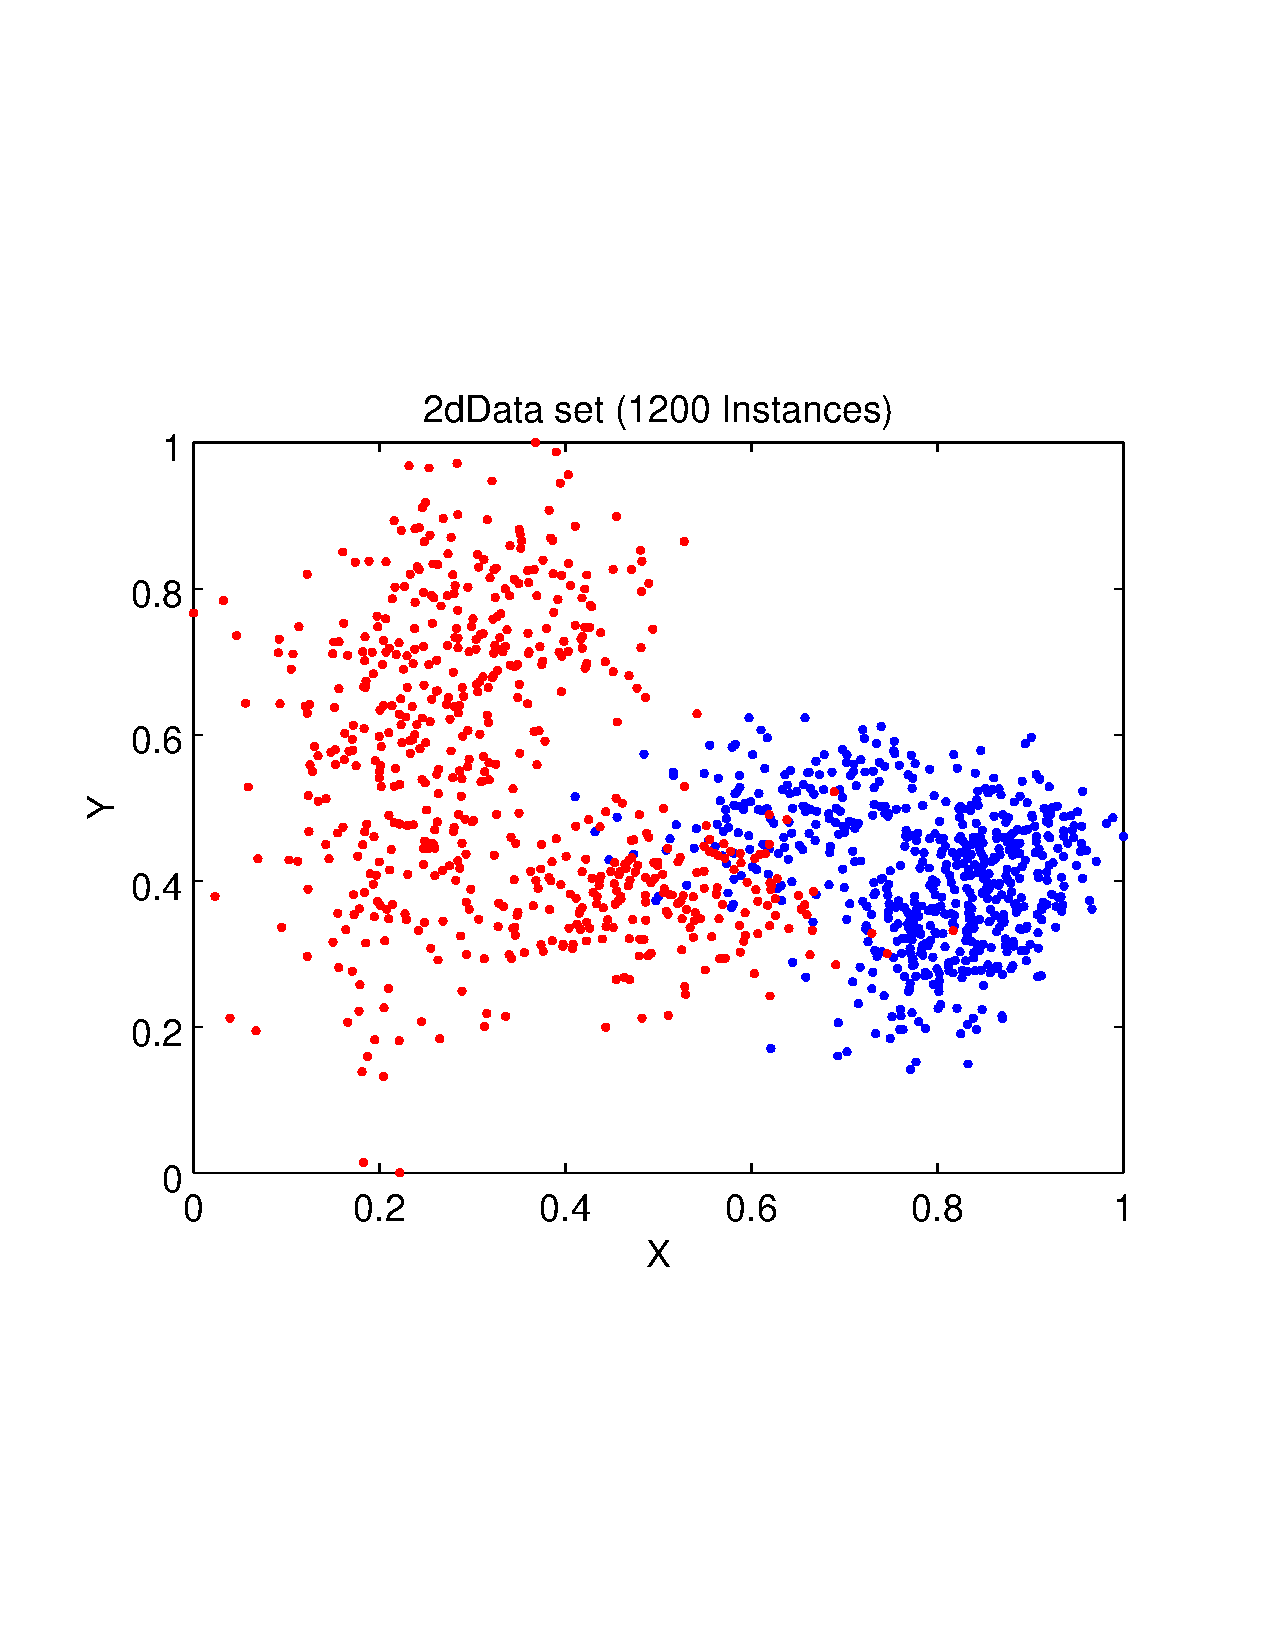
\includegraphics[trim = 0cm 6cm 0cm 5cm, clip = true, width = 0.45\textwidth]{2dDataIllustration}
	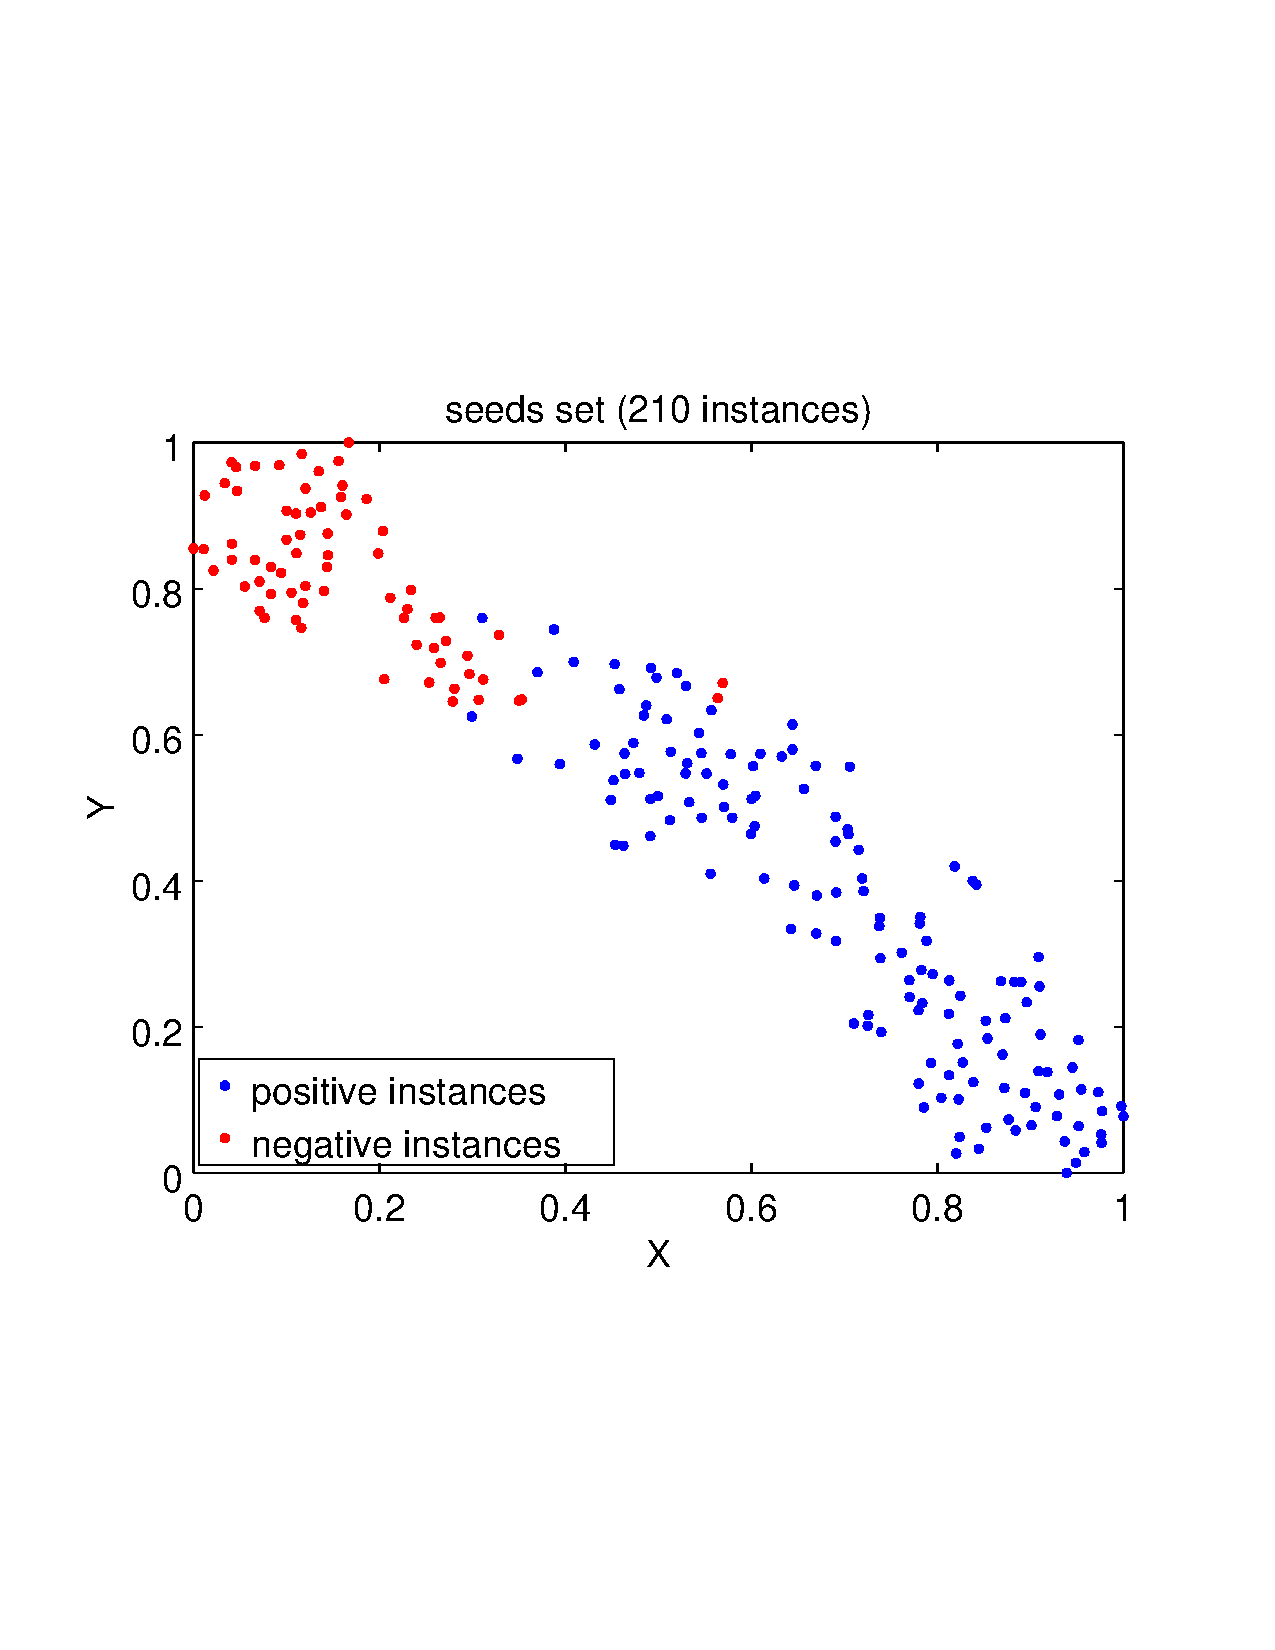
\includegraphics[trim = 0cm 6cm 0cm 5cm, clip = true, width = 0.45\textwidth]{seedsIllustration}
	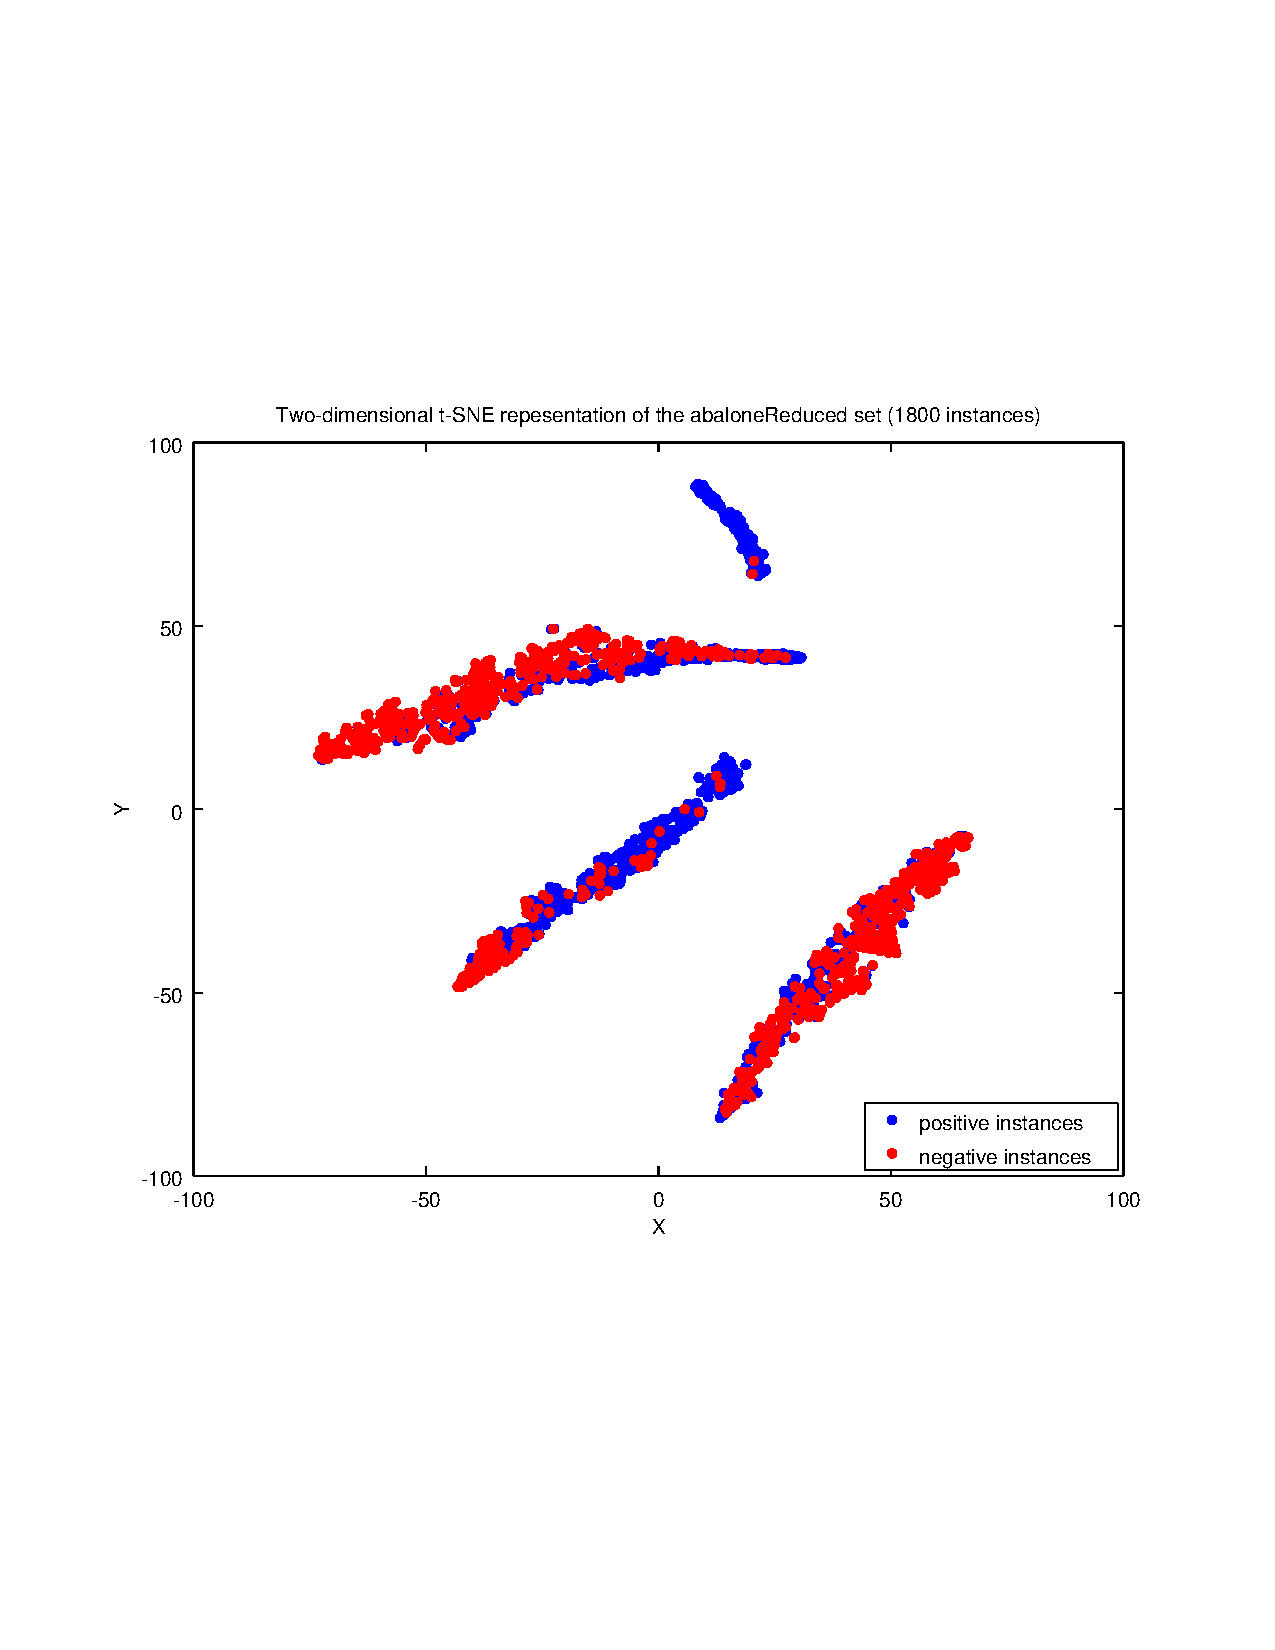
\includegraphics[trim = 0cm 6cm 0cm 5cm, clip = true, width = 0.45\textwidth]{abaloneReducedIllustration}
	\caption{Visualizations of the datasets checke1, 2dData, seeds and a downsized version of abalone \cite{Chapelle2005,KremplEtAl2014,CharytanowiczEtAl2010,NashEtAl1994}.\newline The illustration of seeds and abalone was done using an implementation of t-SNE \cite{vanDerMaaten2008}}
	\label{fig:datasetIllustrations}
\end{figure}

\subsection{Parameters}

Some of the methods as well as the fitting requires the specification of parameters like the number of iterations or error tolerance. As their choice may influence the results, all parameters used will be stated in this section.

For each combination of dataset, active learner and function model, 50 runs were simulated, each with 30 total instances purchased. All function models were fit on the same data.

For the path-based methods, $|X_T|^2$ paths were randomly selected. The required subset performance estimations were computed afterwards. Both averaging methods make use of all subsets up to ~10000 (due to rounding not exact); the bootstrap variant was allowed 50 samples per subset. This cap was placed due to memory limitations. The modified variants with weighting/no-information rate use the same subsets/paths for any given test run. The cross-validation competitor used 5 folds; its bootstrapping counterpart also got 50 bootstrap samples per estimation.

All curves were fit with the Levenberg-Marquardt algorithm, even the linear model; this was done to normalize the testing environment. The ranges for initial parameters as well as their bounds can be seen in \ref{tab:functionParams}. Each fitting can use up to 300 iterations with a scalar tolerance of $10^{-4}$, i.e. if the sum of squared errors is lower than $0.0001$, the fitting is considered done and will not use the remaining iterations. The partial derivatives were provided, thus numeric derivation was not necessary.

\begin{table}[h]
	\begin{tabular}{c | c | c | c}
	\textbf{Function model} & \textbf{Equation} & \textbf{Parameter bounds} & \textbf{Initial parameter range} \\
	\hline
	3-Exponential & $f_E(x) = a + b \cdot e^{c \cdot x}$ & \begin{tabular}{l}$a \in [0,1]$ \\ $b \in [-\infty, 0]$ \\ $c \in [-\infty, 0]$\end{tabular} & \begin{tabular}{l}$a \in [0,1]$ \\ $b \in [-2, 0]$ \\ $c \in [-2, 0]$\end{tabular} \\
	\hline
	Sigmoid & $f_S(x) = a + b \cdot e^{c \cdot x}$ & \begin{tabular}{l}$a \in [0,1]$ \\ $b \in [-\infty, 0]$ \\ $c \in [-\infty, 0]$\end{tabular} & \begin{tabular}{l}$a \in [0,1]$ \\ $b \in [-2, 0]$ \\ $c \in [-2, 0]$\end{tabular} \\
	\hline
	Linear & $f_L(x) = a + b \cdot x$ & \begin{tabular}{l}$a \in [0,1]$ \\ $b \in [0, \infty]$\end{tabular} & \begin{tabular}{l}$a \in [0,1]$ \\ $b \in [0, 4]$\end{tabular} \\
	\end{tabular}
	\caption{Function-specific parameters for model fitting}
	\label{tab:functionParams}
\end{table}

As Levenberg-Marquardt may be stuck in local minima or not converge at all, each fitting was done 5 times with random parameters drawn from their respective ranges to attempt to circumvent these hazards. Then, the fit with the lowest sum of squared errors w.r.t. the data given was selected. If the fitting used statistical weights, they were also used in this selection.

The reference accuracy was obtained by using holdout test sets, each randomly selected with the same size as the classifier's training set. The classifier in question then assigned a class label and the accuracy is computed for each of the holdout sets. Both variance and mean are obtained from the accuracies of all holdout sets and then used to construct a beta distribution; the mean is also used in the traditional error computation.

\section{Test results}

Due to the sheer amount of data, we will only cover a portion of the generated graphs. To help keeping an overview, we structure the evaluation into various parts: first, we take a look at the summed mean error for unweighted fitting with the exponential model and the traditional ones to get an idea of the bias each methods brings with it. Then we evaluate the spread of the estimates by inspecting the summed squared error. Then we take a look at the influence of the weighting on each method as well as that of the different function models. Next come the distribution comparisons; they are limited to a subset of methods anyway and will not cover every setting of the tests. Last, we will take a look at the computation time required for each method.

\subsection{Error measures}

To inspect whether our estimators carry a bias and if yes, how large it is, we compute the mean error between the holdout accuracy and that of our methods for each training set size and test run. Since some stages of the learning process may be easier for the estimators than others we group the error by the set size they were measured for. \ref{fig:meanErrorBars} shows the summed mean error for the training set sizes from $3-7$, $8-15$ and $16-30$.

\begin{figure}[h]
	\centering
	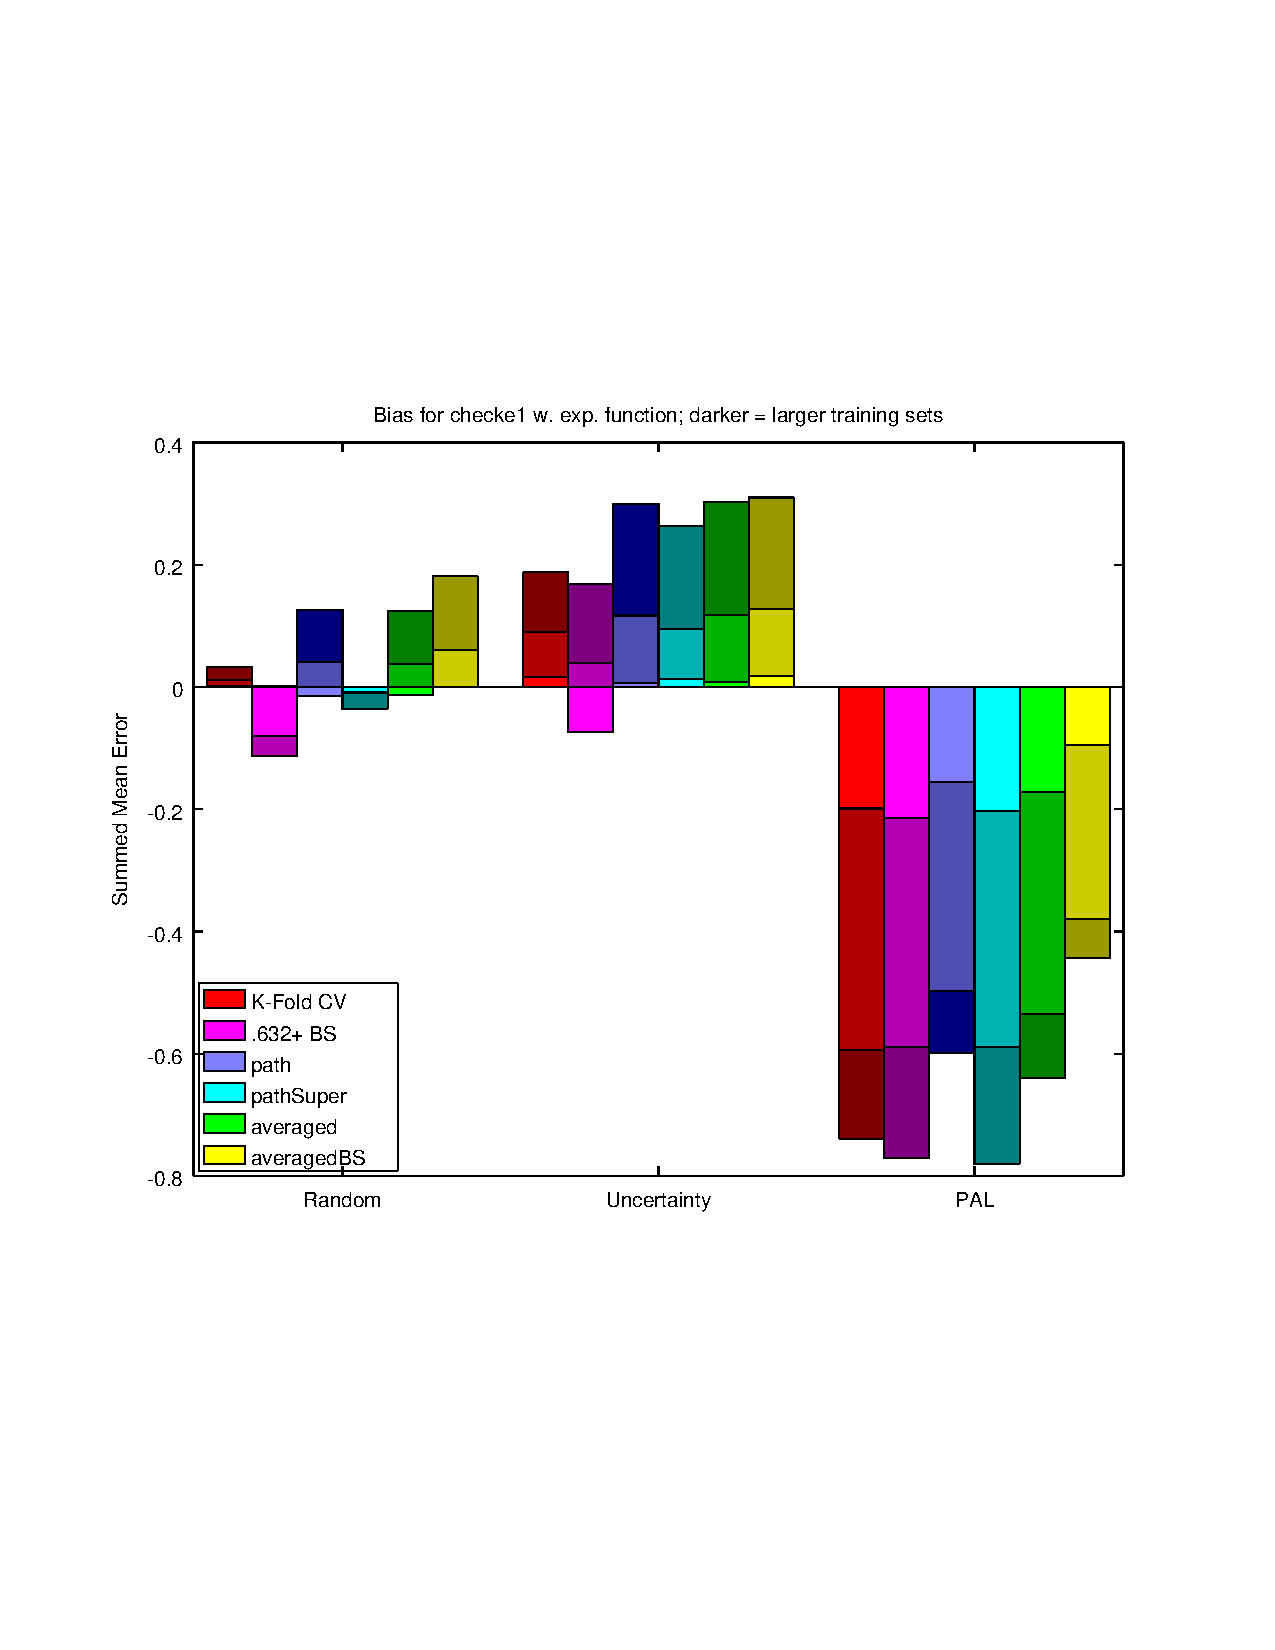
\includegraphics[trim = 1.5cm 6cm 2.5cm 6cm, clip = true, width = 0.48\textwidth]{meanErrchecke1}
	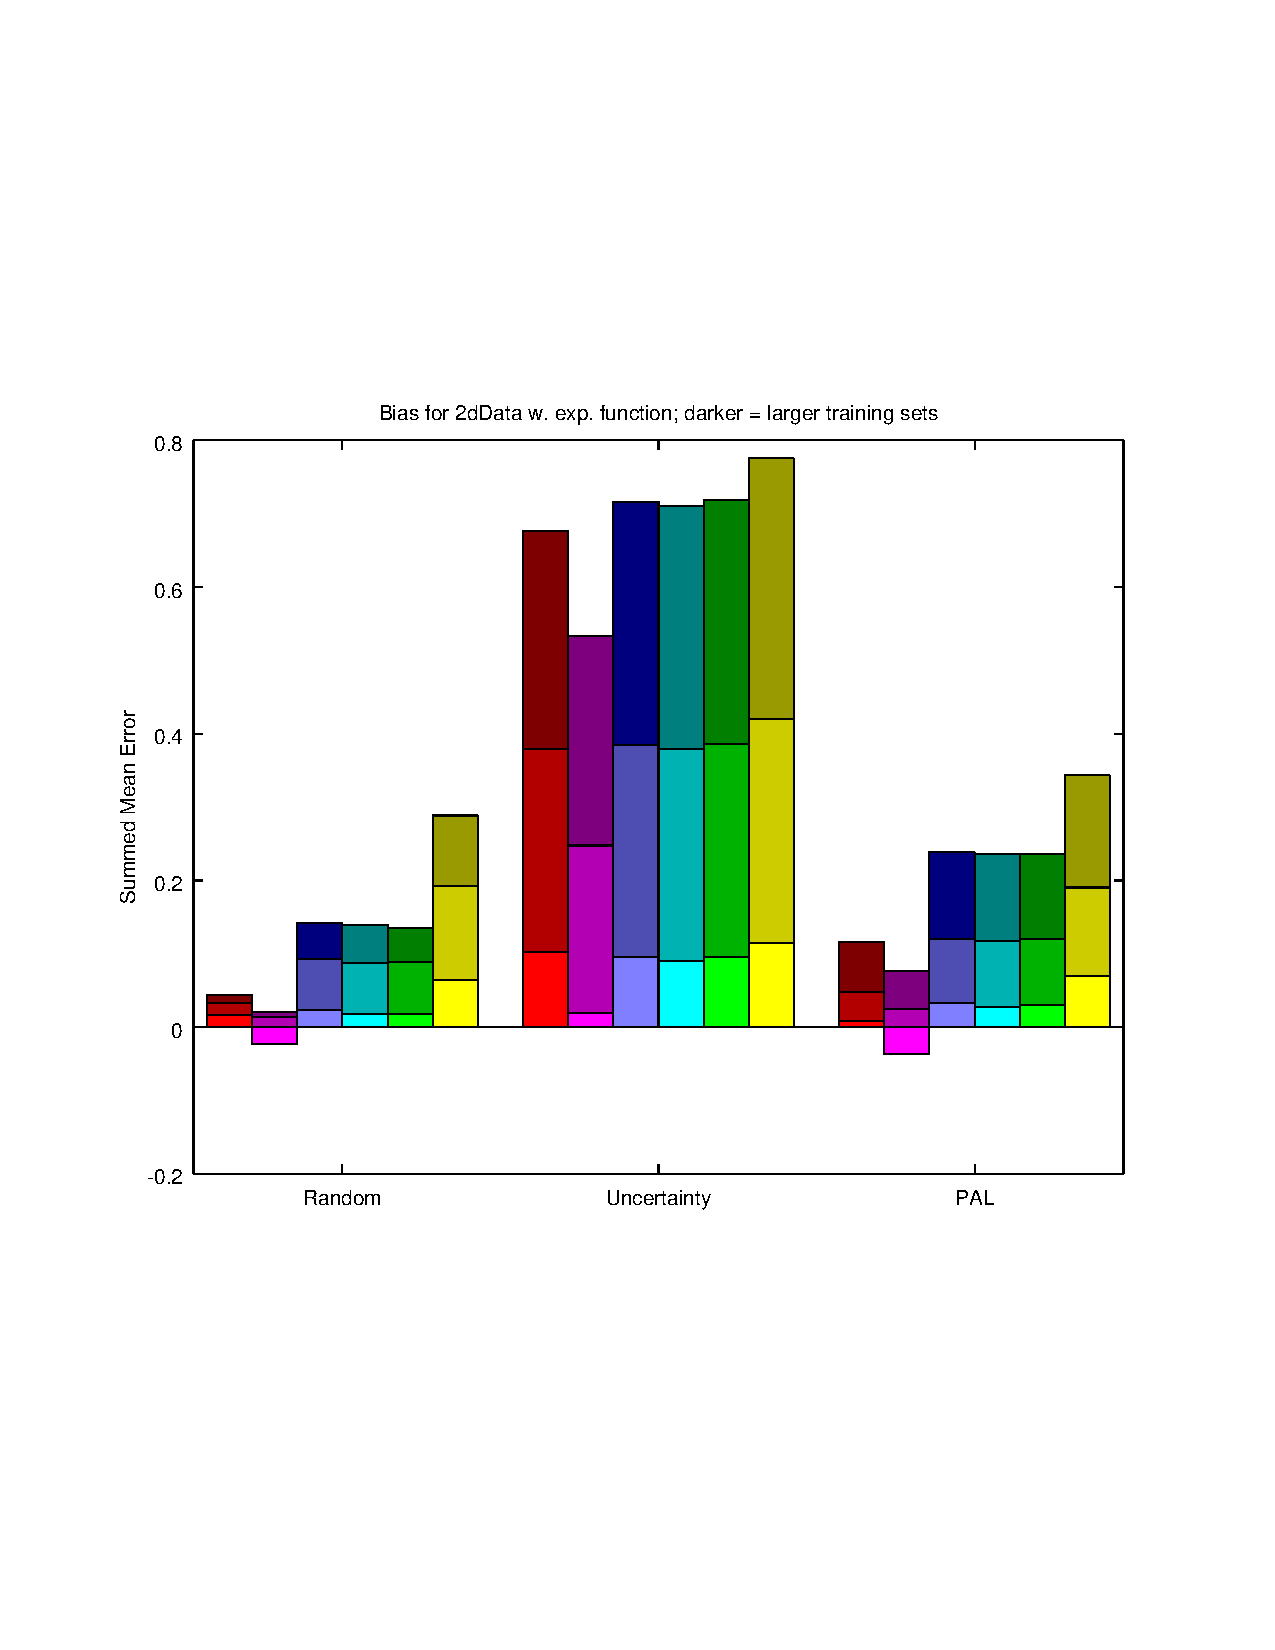
\includegraphics[trim = 1.5cm 6cm 2.5cm 6cm, clip = true, width = 0.48\textwidth]{meanErr2dData}
	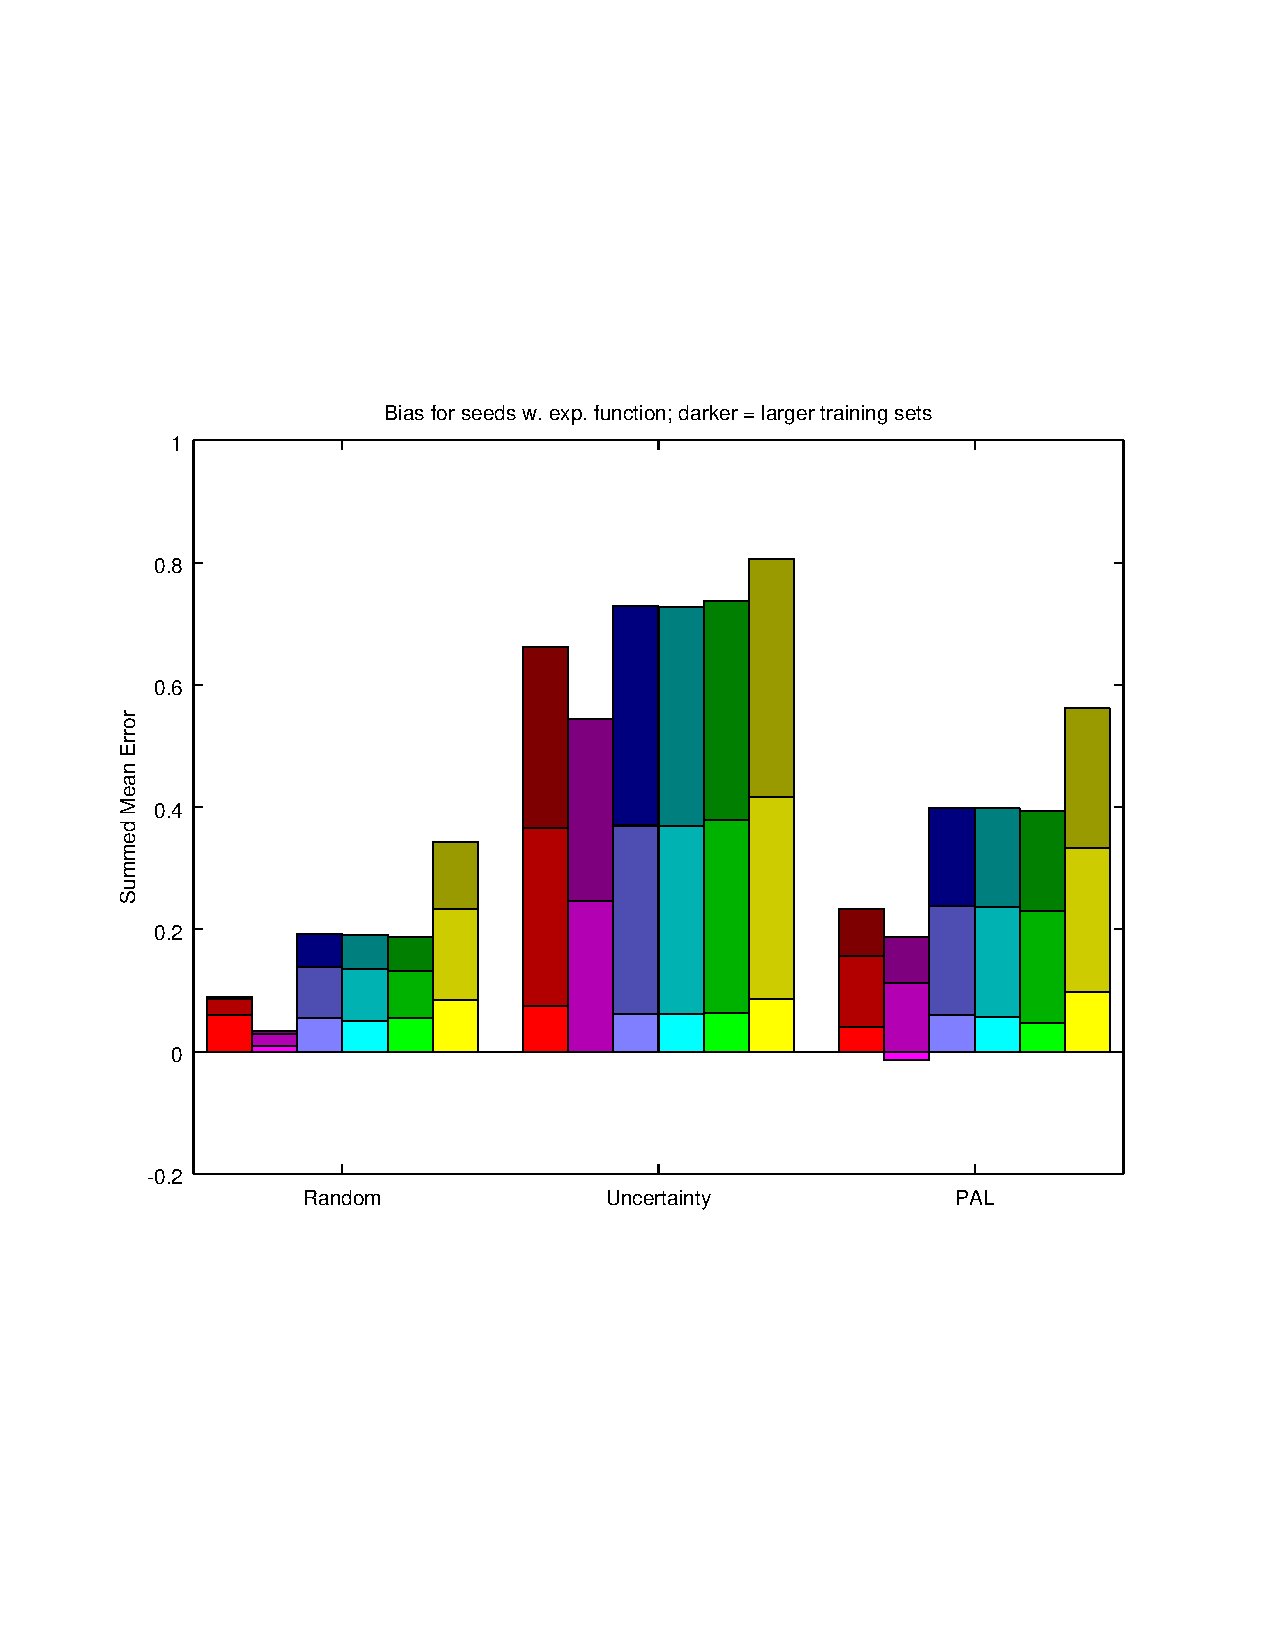
\includegraphics[trim = 1.5cm 6cm 2.5cm 6cm, clip = true, width = 0.48\textwidth]{meanErrseeds}
	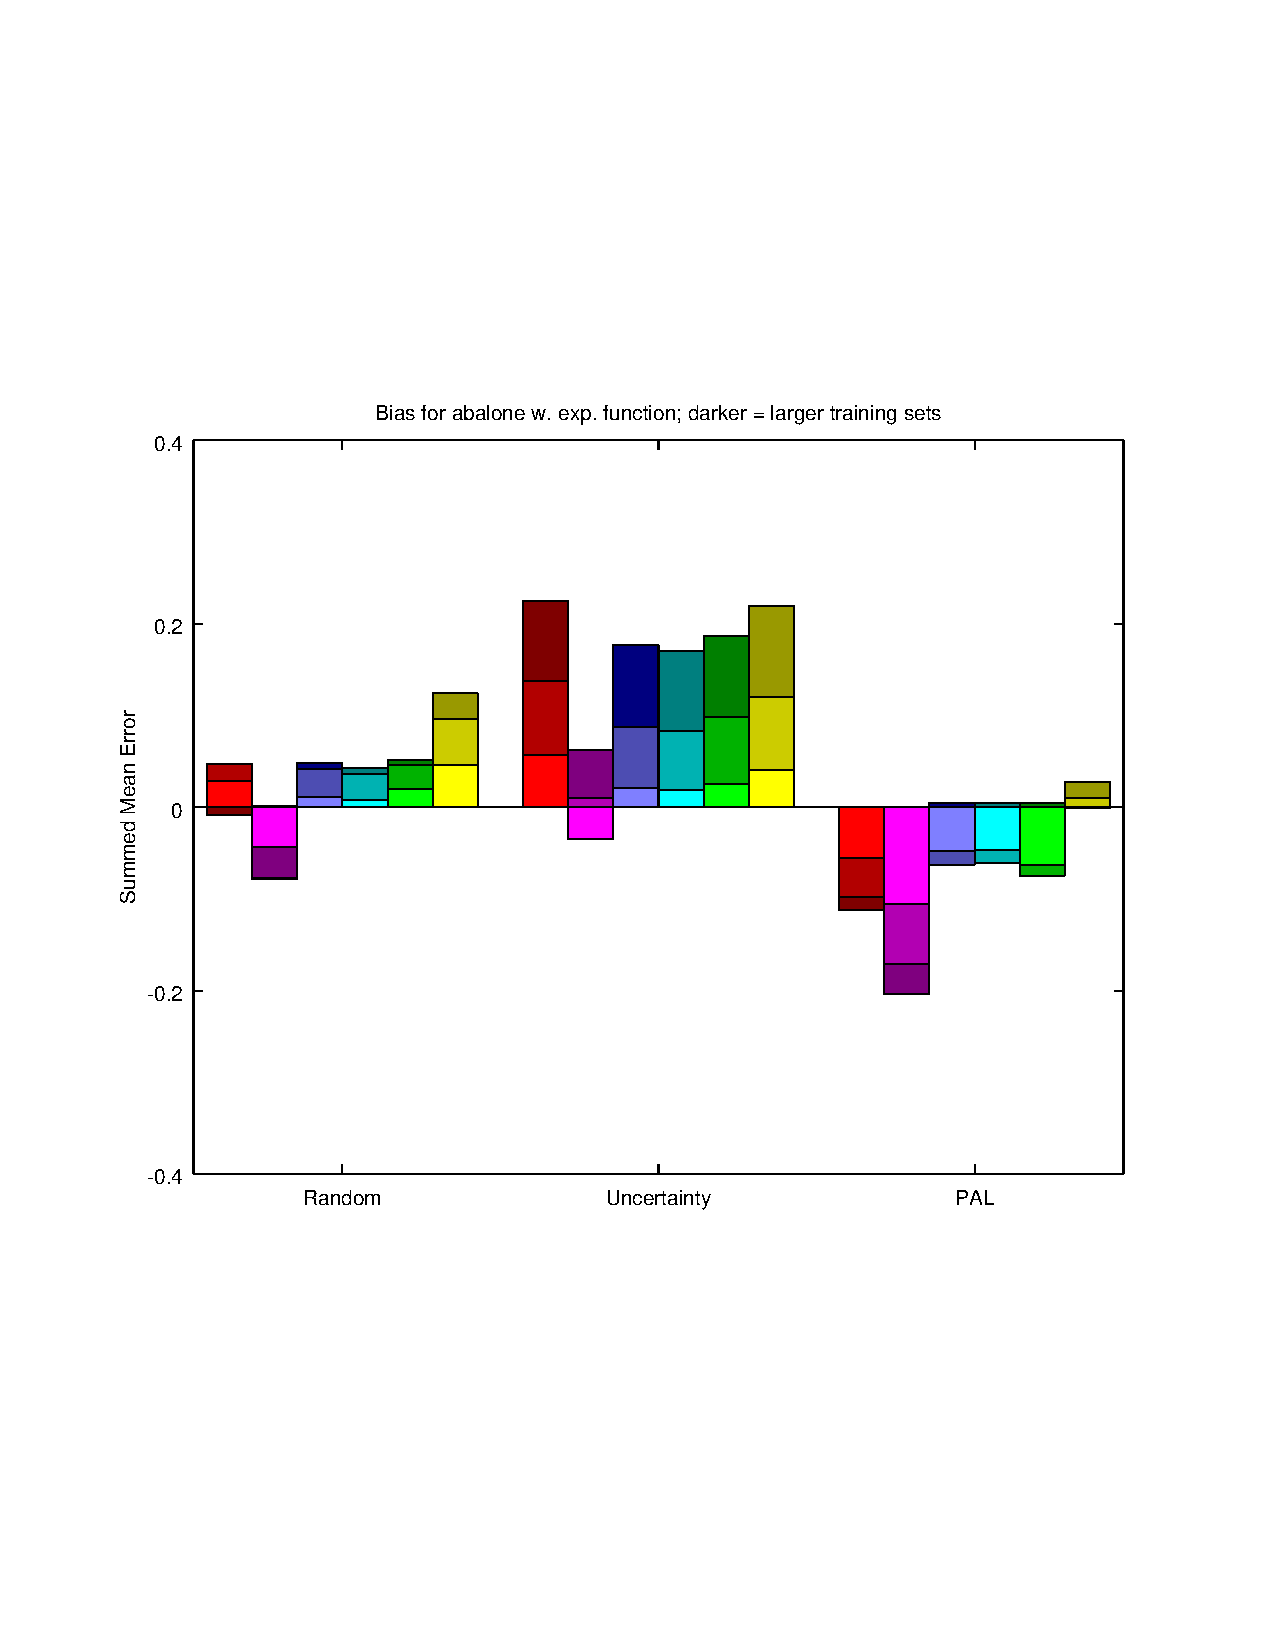
\includegraphics[trim = 1.5cm 6cm 2.5cm 6cm, clip = true, width = 0.48\textwidth]{meanErrabalone}
	\caption{Summed mean errors for the different active learners and datasets using the exponential model}
	\label{fig:meanErrorBars}
\end{figure}



\begin{figure}[h]
	\centering
	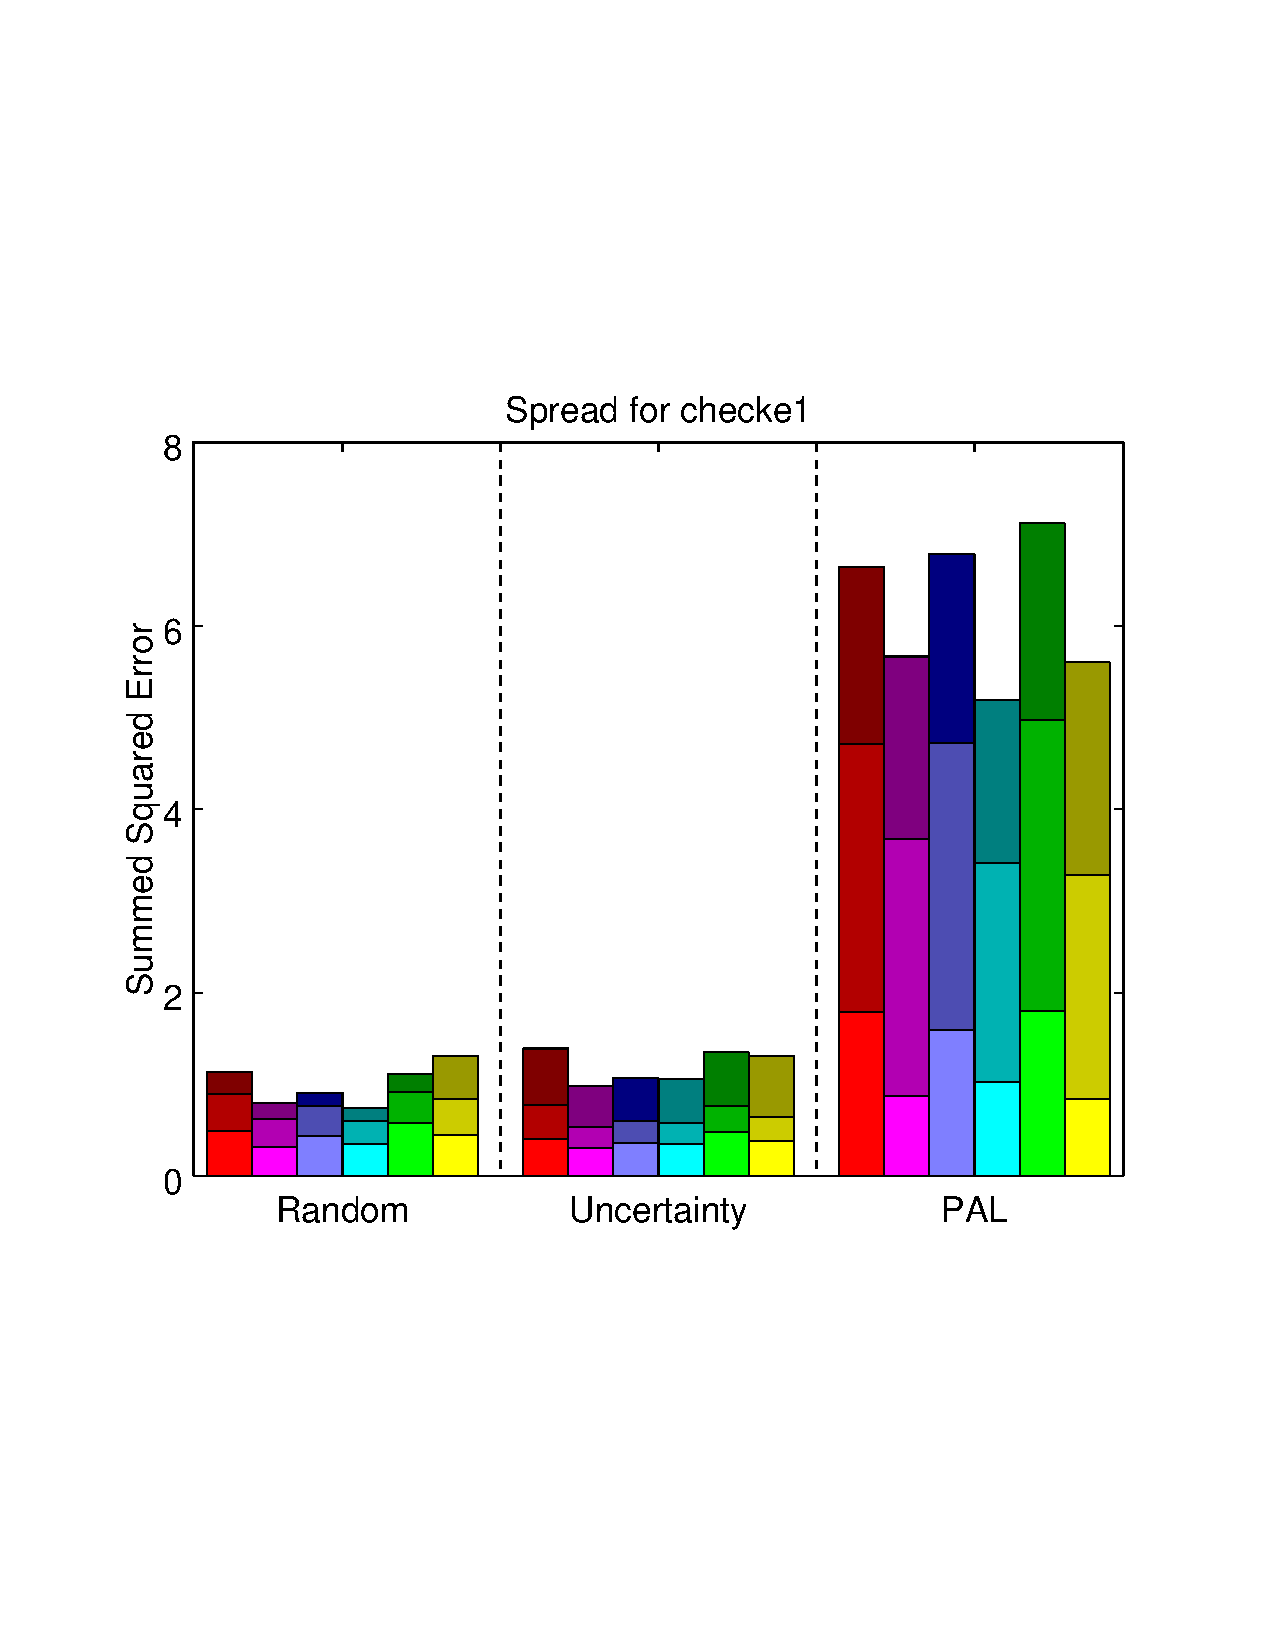
\includegraphics[trim = 1.5cm 6cm 2.5cm 6cm, clip = true, width = 0.48\textwidth]{squErrchecke1}
	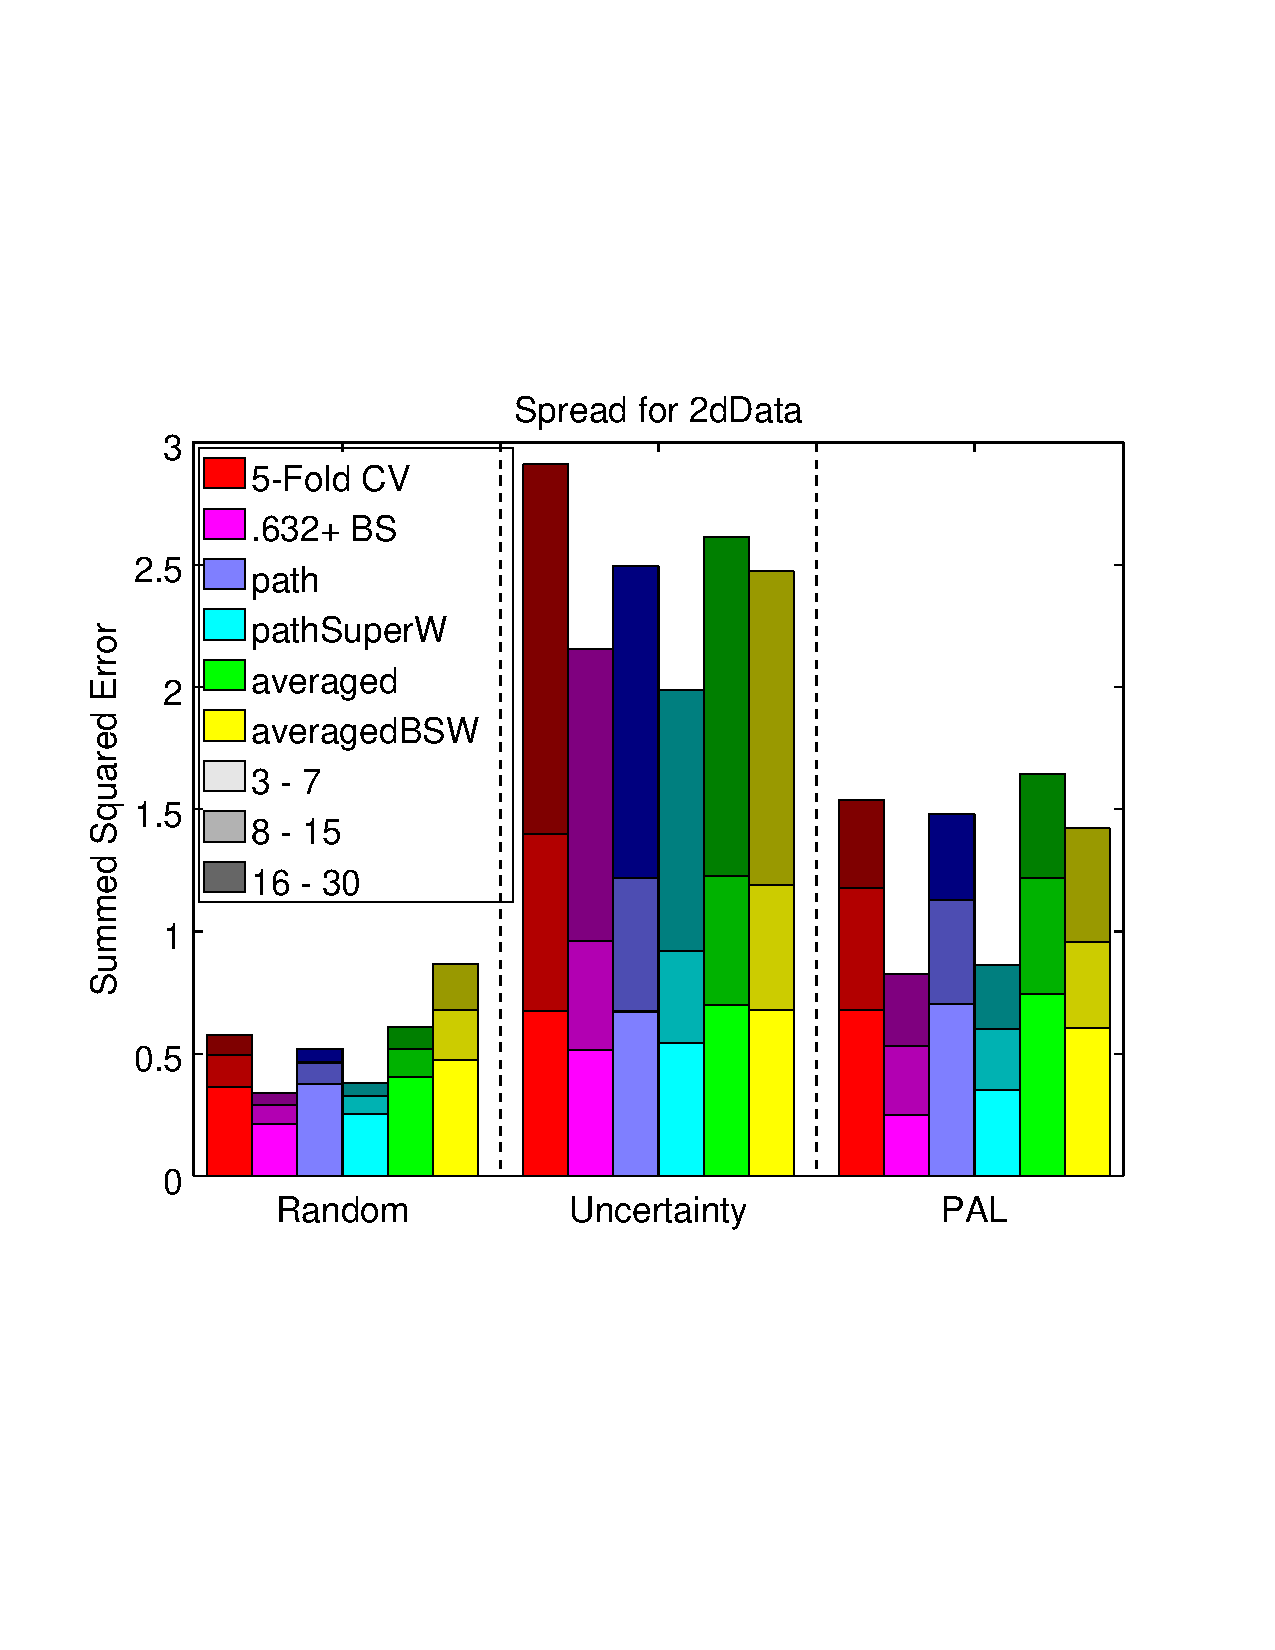
\includegraphics[trim = 1.5cm 6cm 2.5cm 6cm, clip = true, width = 0.48\textwidth]{squErr2dData}
	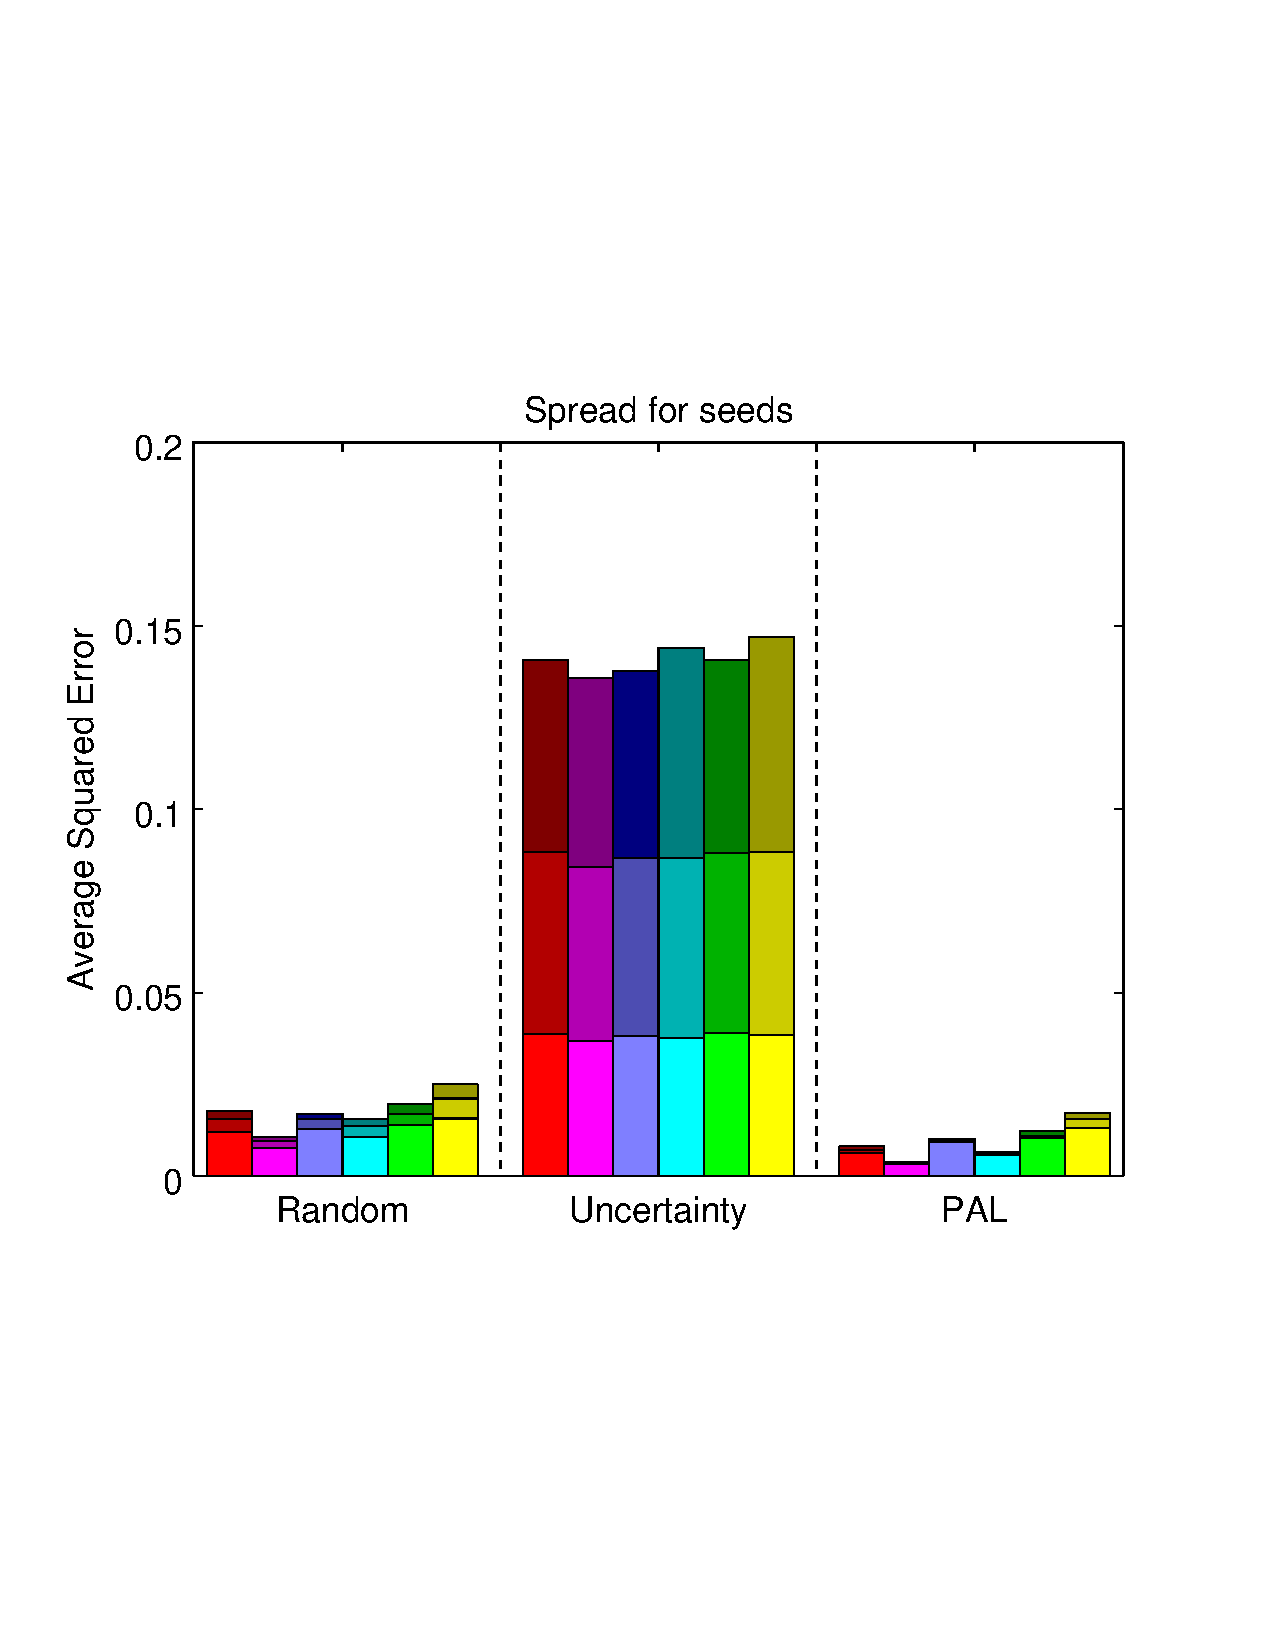
\includegraphics[trim = 1.5cm 6cm 2.5cm 6cm, clip = true, width = 0.48\textwidth]{squErrseeds}
	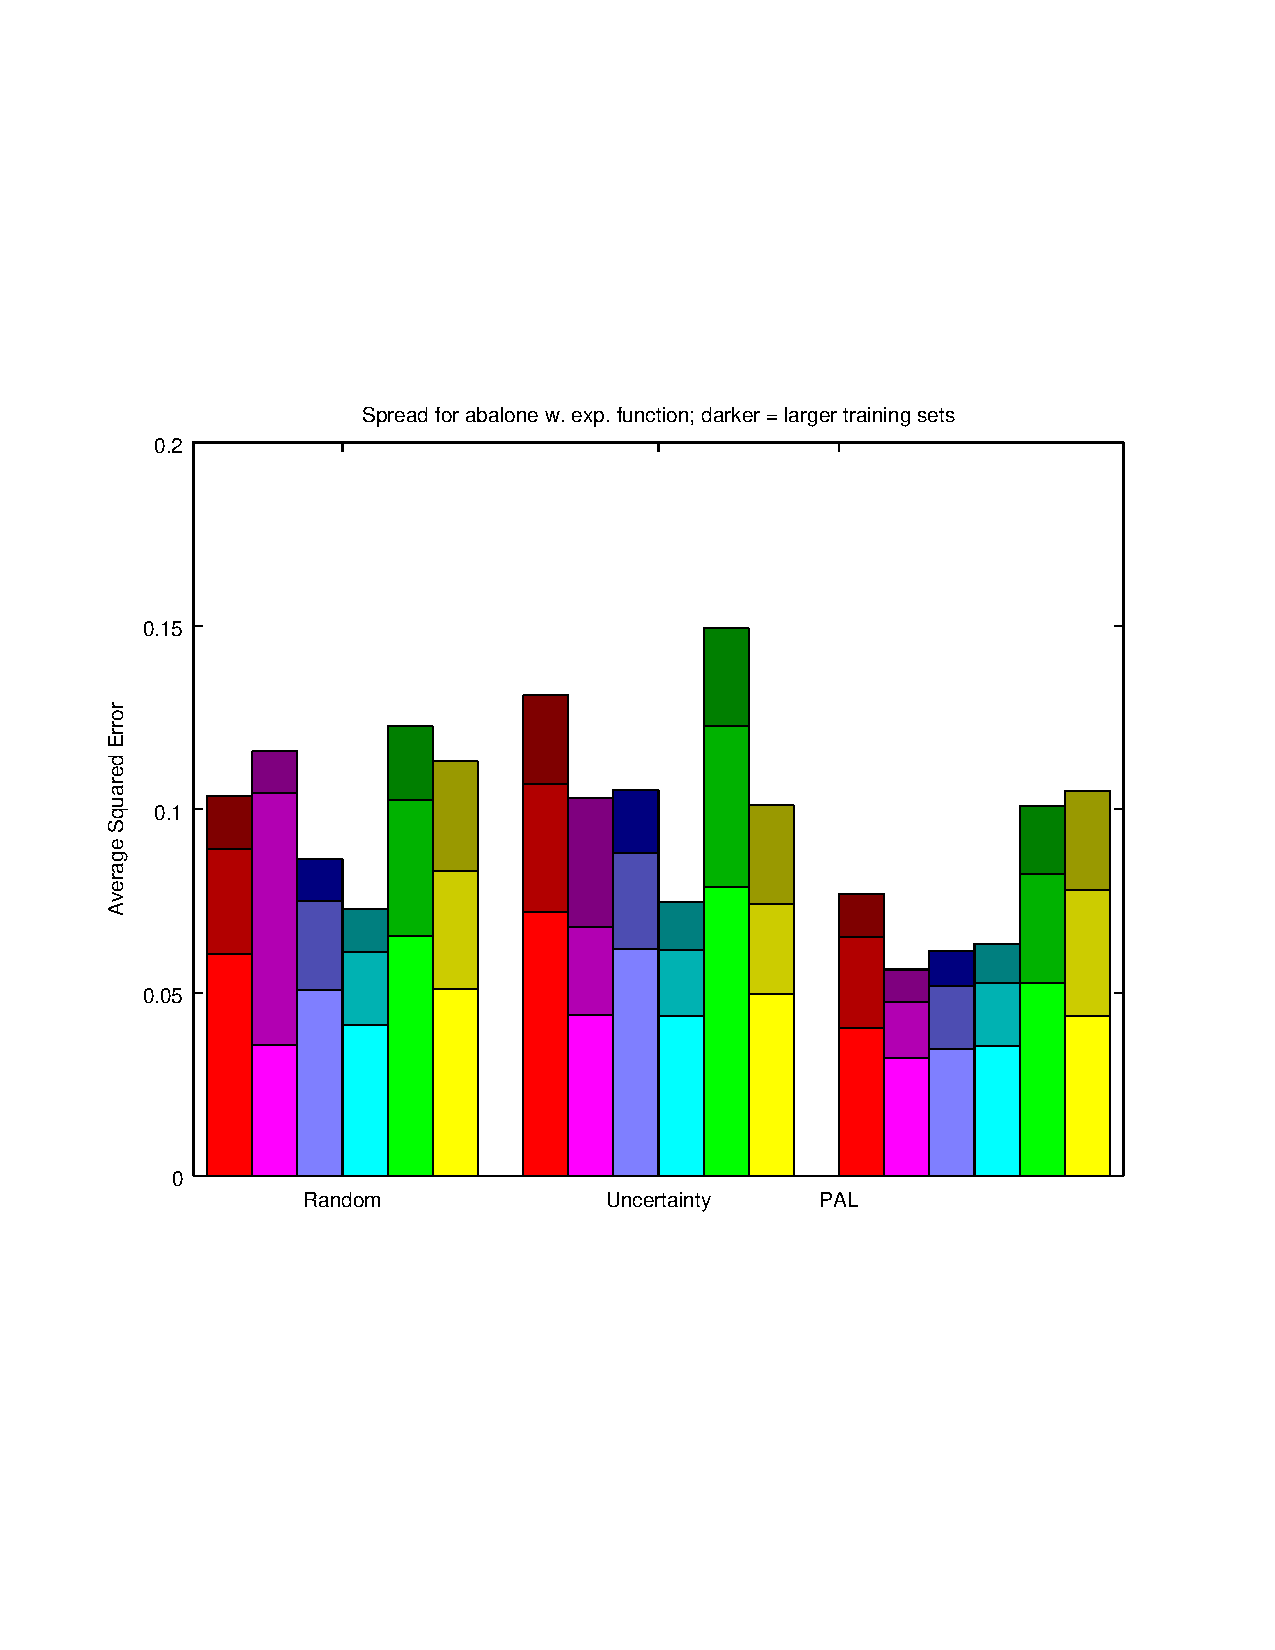
\includegraphics[trim = 1.5cm 6cm 2.5cm 6cm, clip = true, width = 0.48\textwidth]{squErrabalone}
	\caption{Summed squared errors for the different active learners, function models and datasets}
	\label{fig:squaredErrorBars}
\end{figure}


\begin{figure}[h]
	\centering
	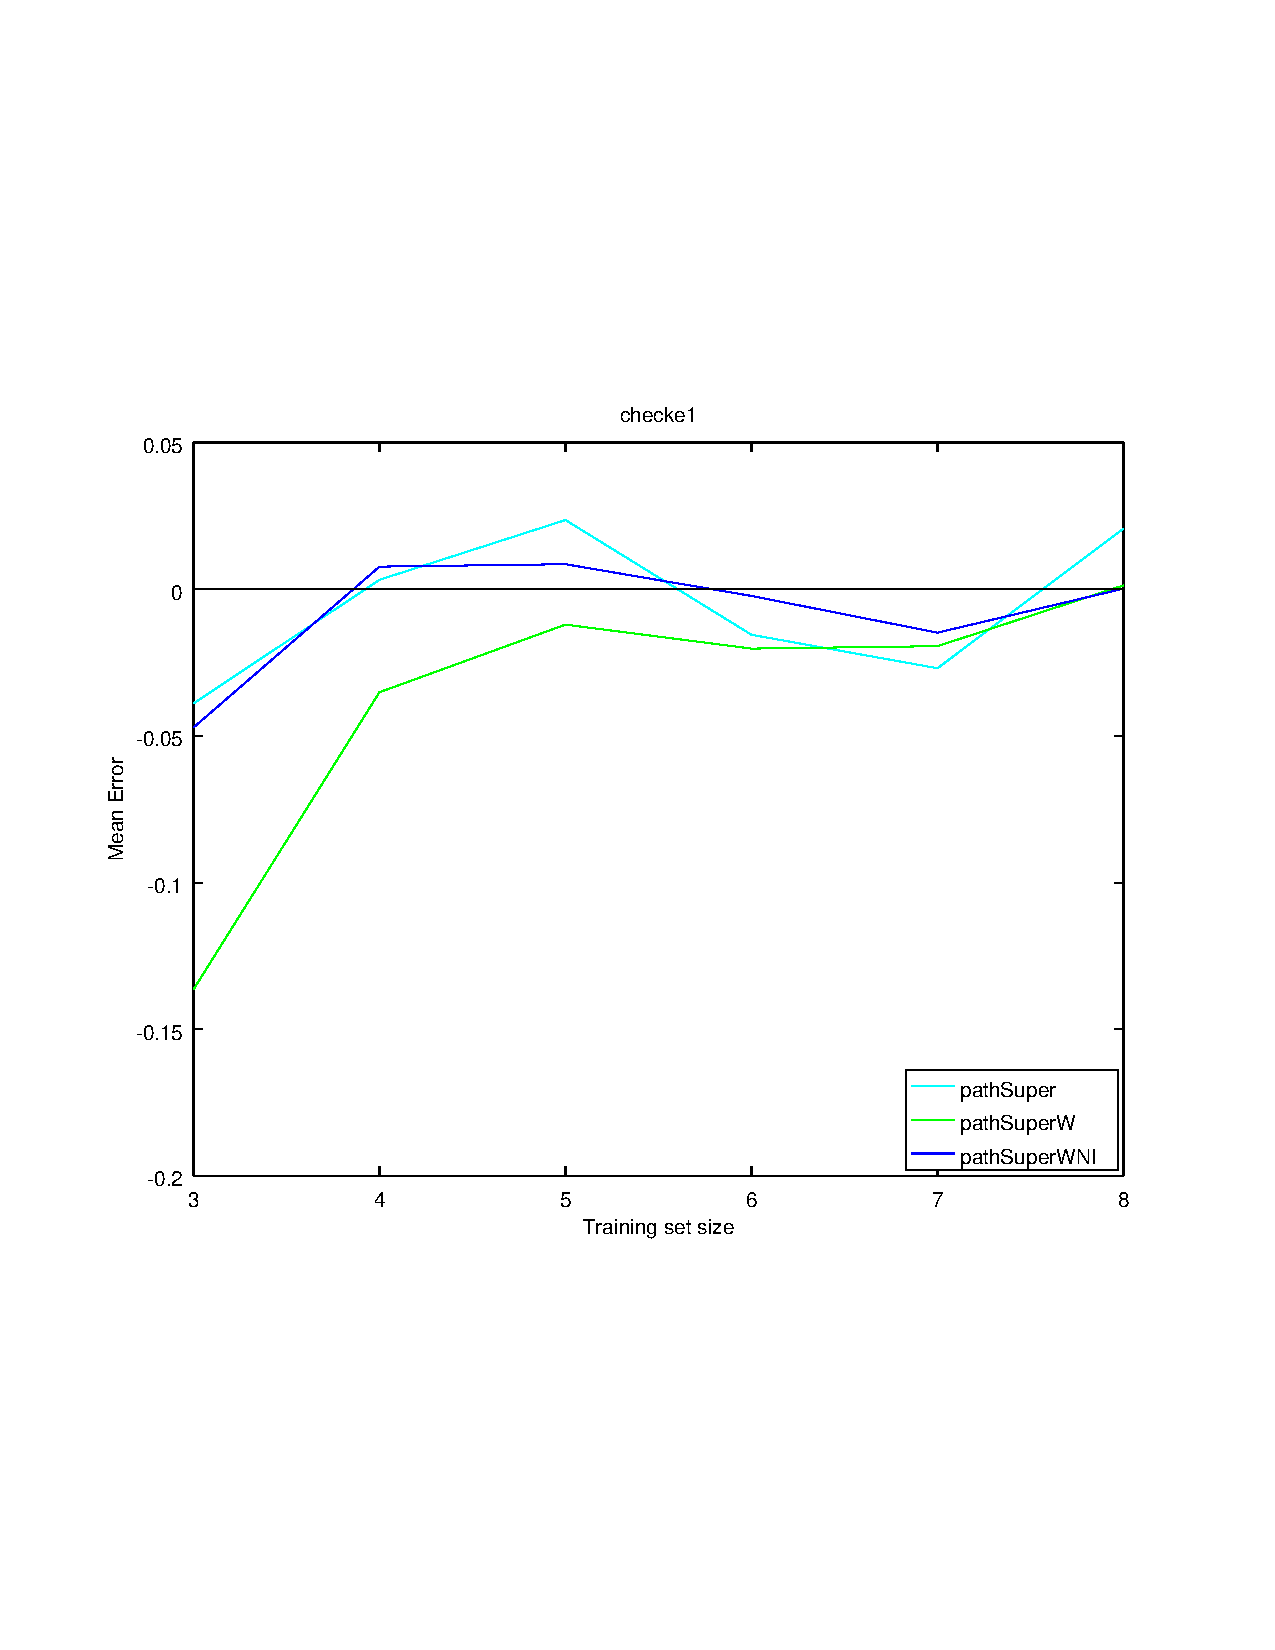
\includegraphics[trim = 1.5cm 6cm 2.5cm 6cm, clip = true, width = 0.48\textwidth]{meanErrLowIterchecke1}
	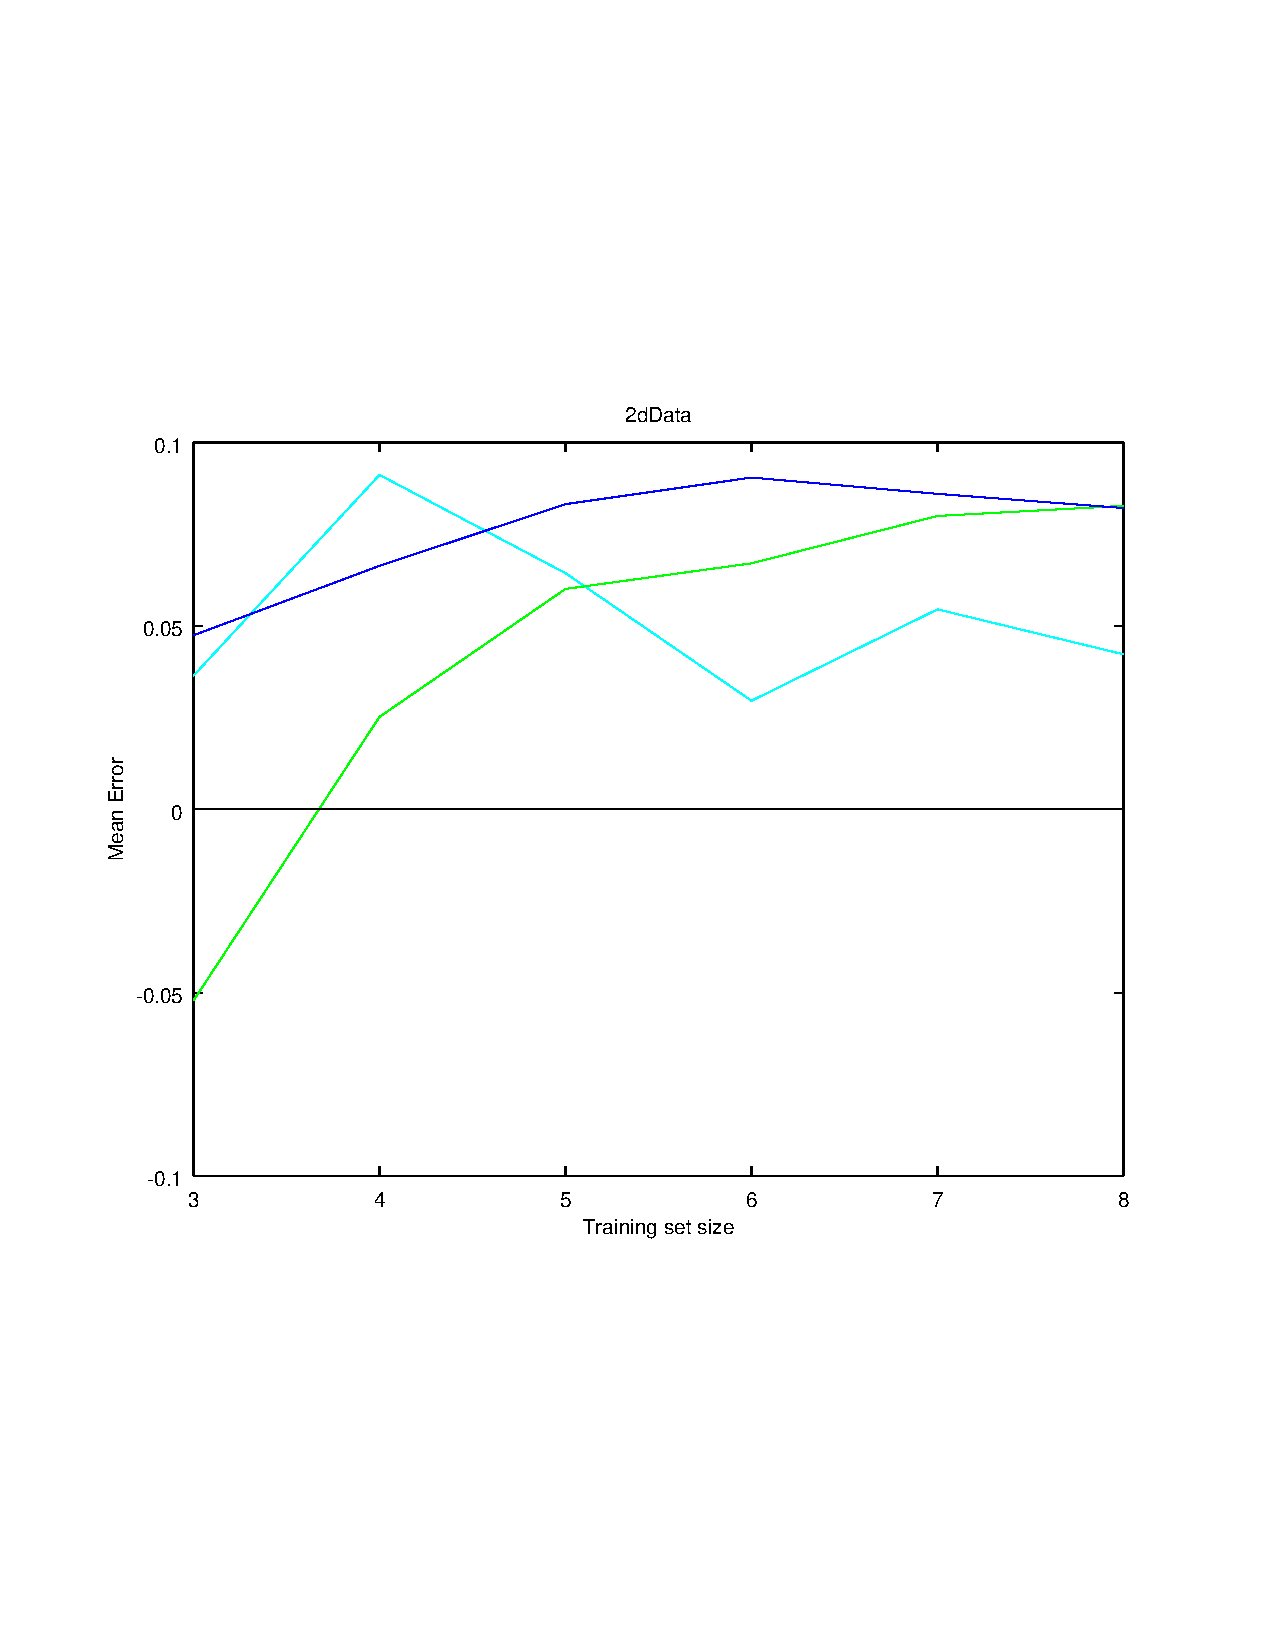
\includegraphics[trim = 1.5cm 6cm 2.5cm 6cm, clip = true, width = 0.48\textwidth]{meanErrLowIter2dData}
	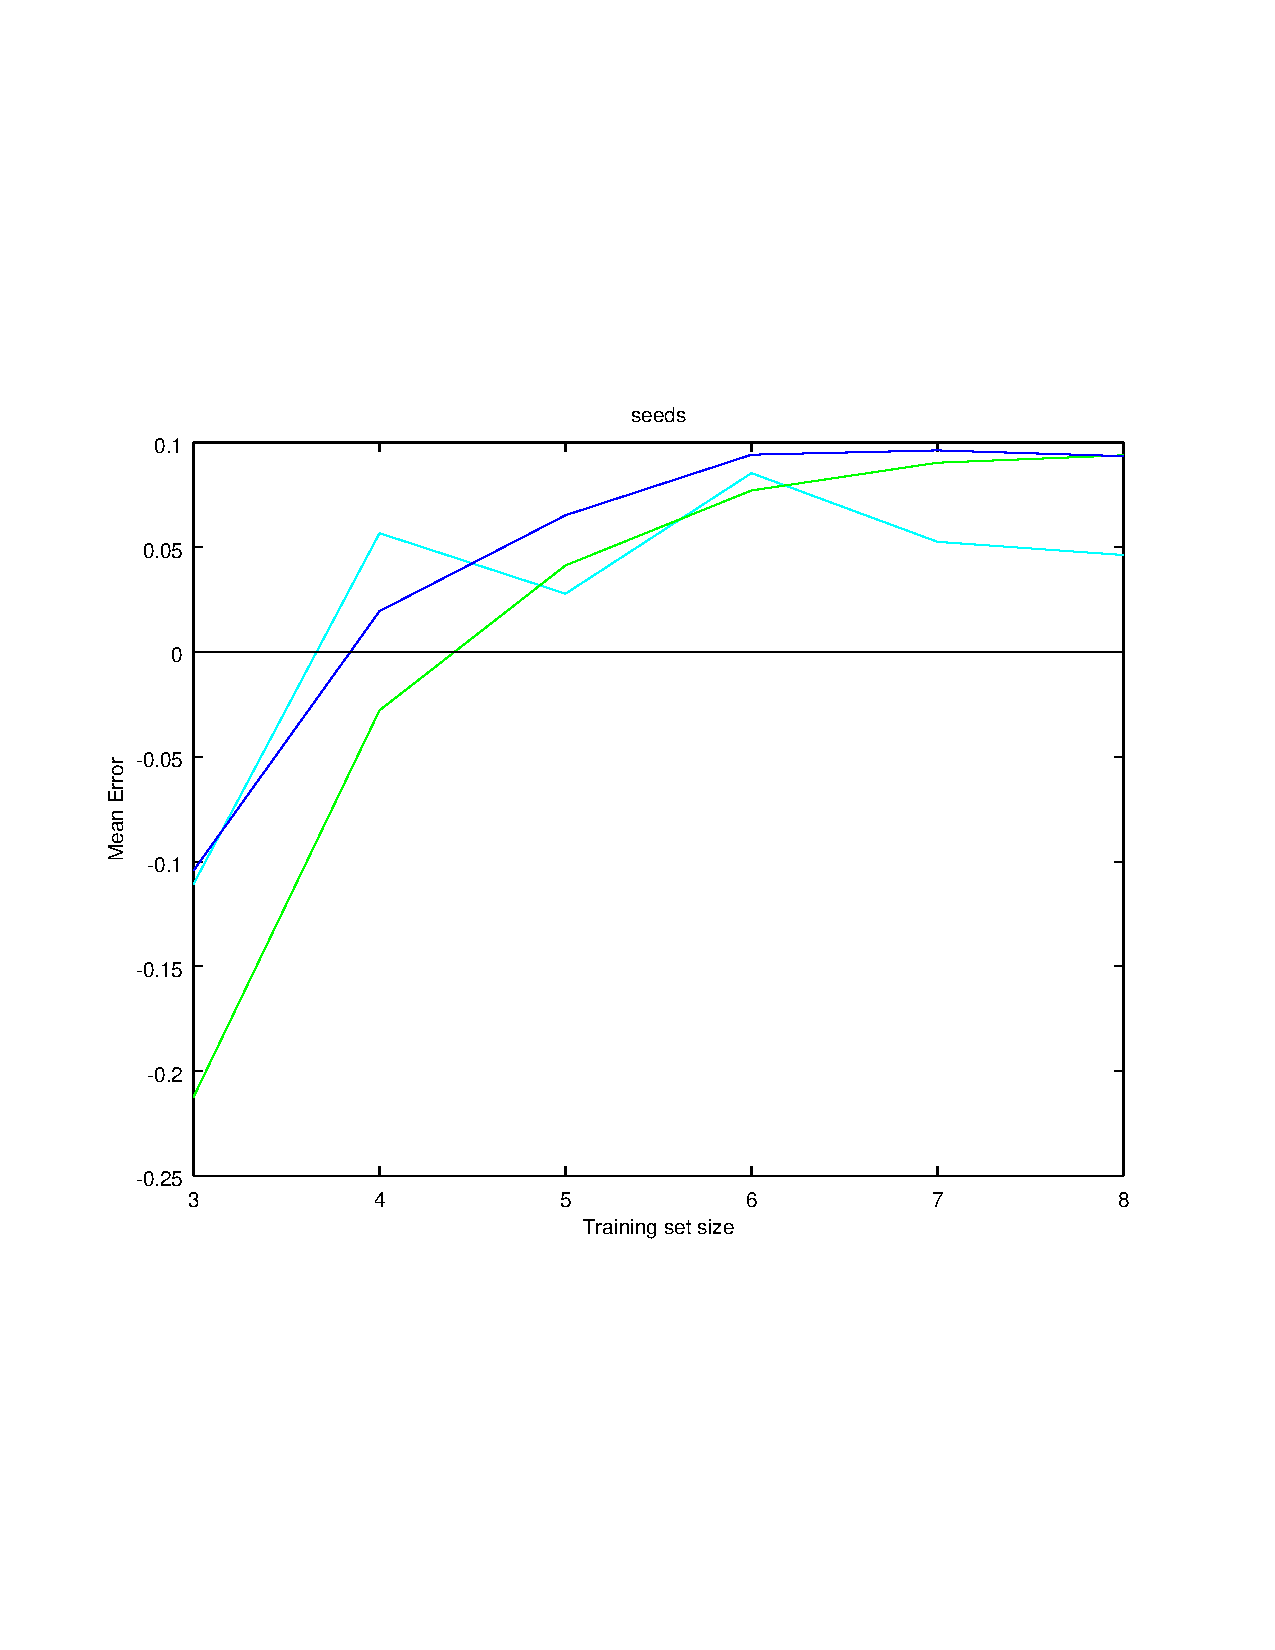
\includegraphics[trim = 1.5cm 6cm 2.5cm 6cm, clip = true, width = 0.48\textwidth]{meanErrLowIterseeds}
	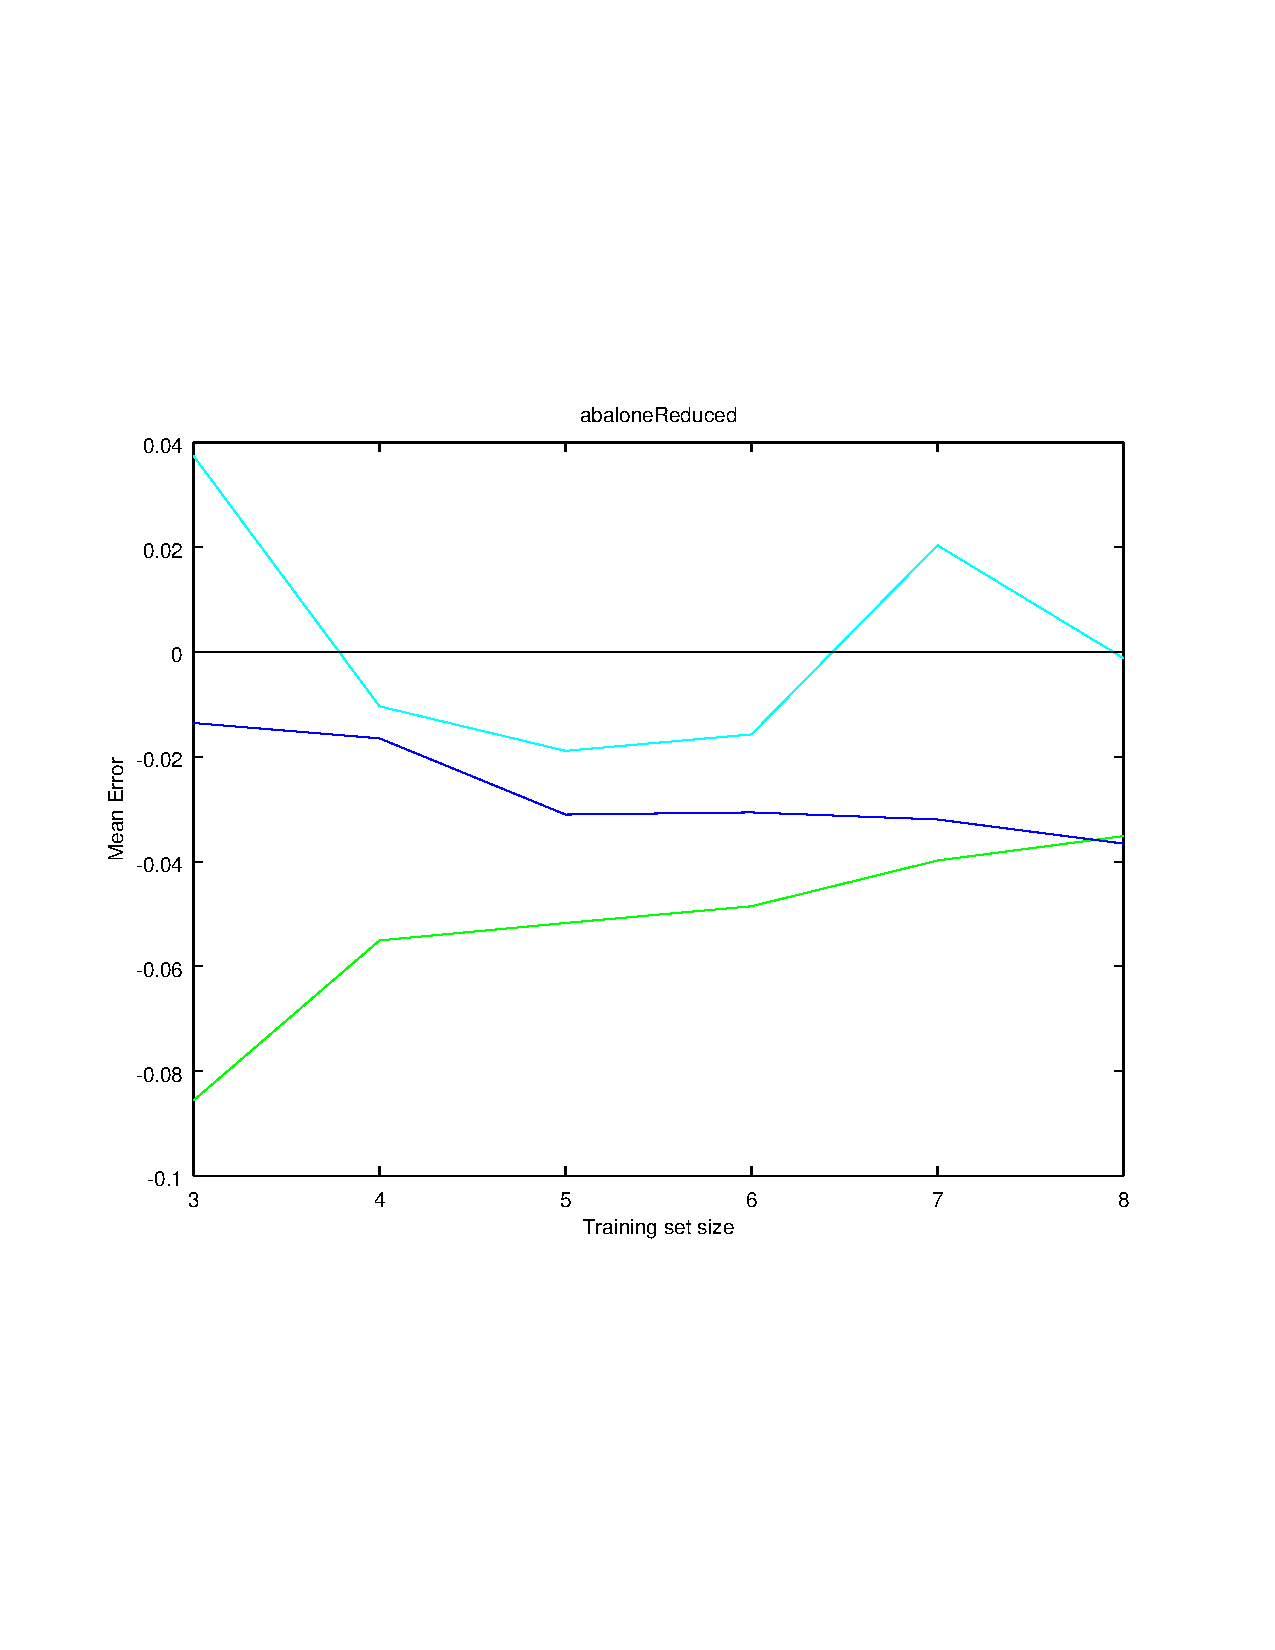
\includegraphics[trim = 1.5cm 6cm 2.5cm 6cm, clip = true, width = 0.48\textwidth]{meanErrLowIterabaloneReduced}
	\caption{Mean error of the three \textit{pathSuper}-methods for small training sets (random sampling, exponential function model)}
	\label{fig:meanErrorLowIter}
\end{figure}

\subsection{Kullback-Leibler divergence}

\begin{figure}[h]
	\centering
	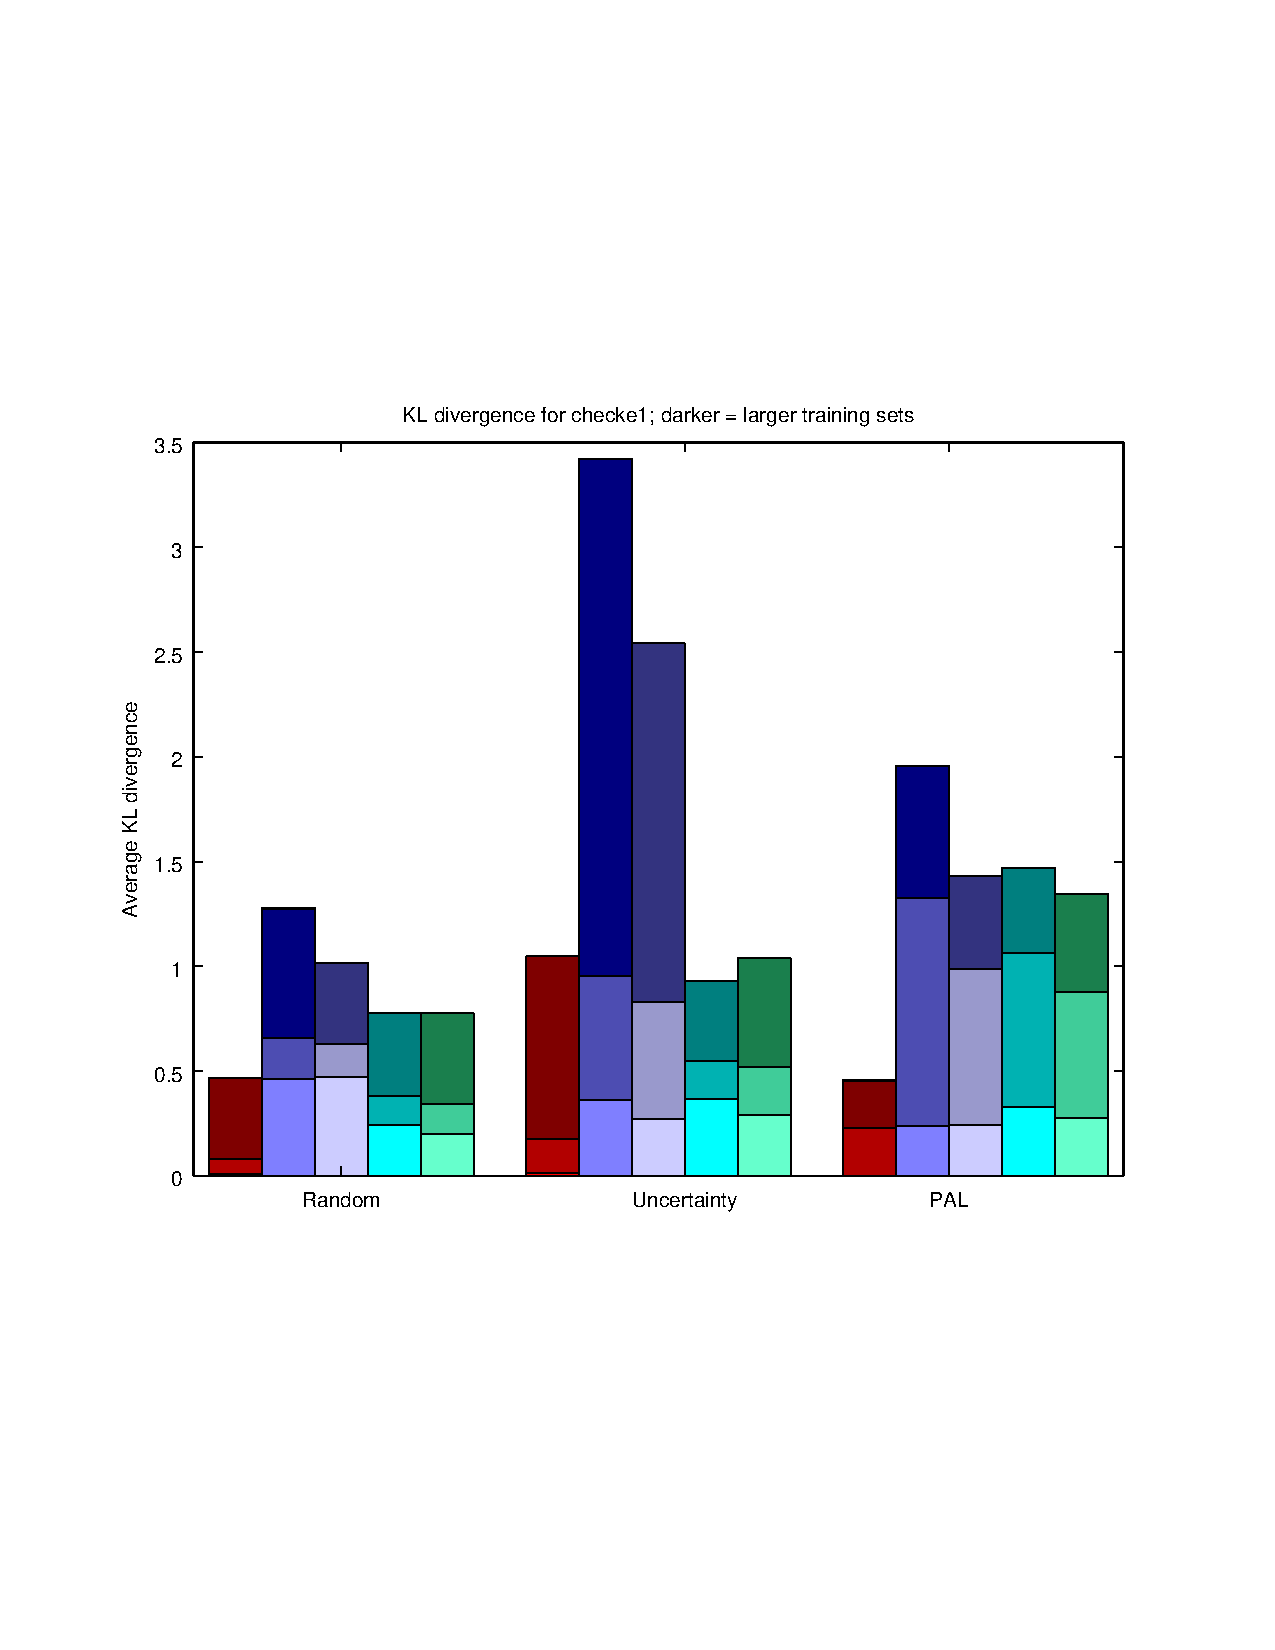
\includegraphics[trim = 1.5cm 6cm 2.5cm 6cm, clip = true, width = 0.48\textwidth]{klDivchecke1}
	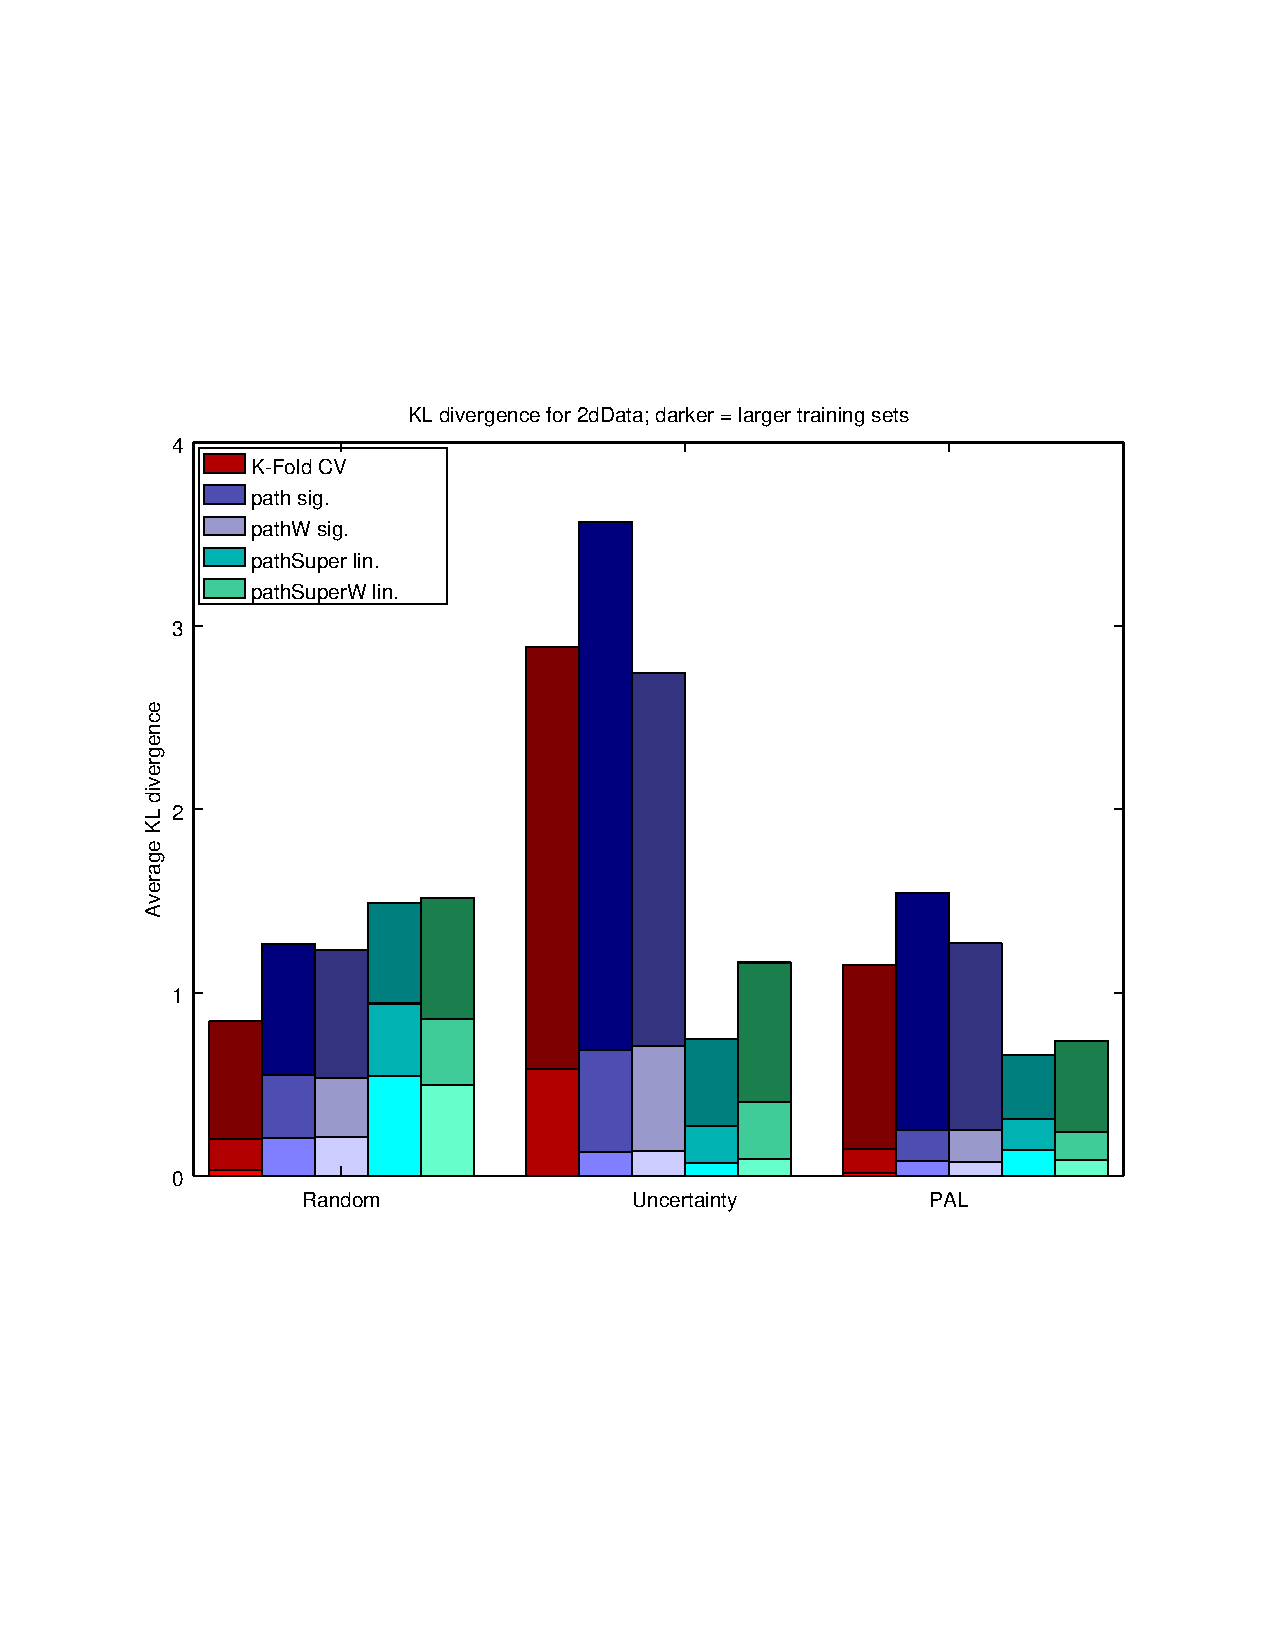
\includegraphics[trim = 1.5cm 6cm 2.5cm 6cm, clip = true, width = 0.48\textwidth]{klDiv2dData}
	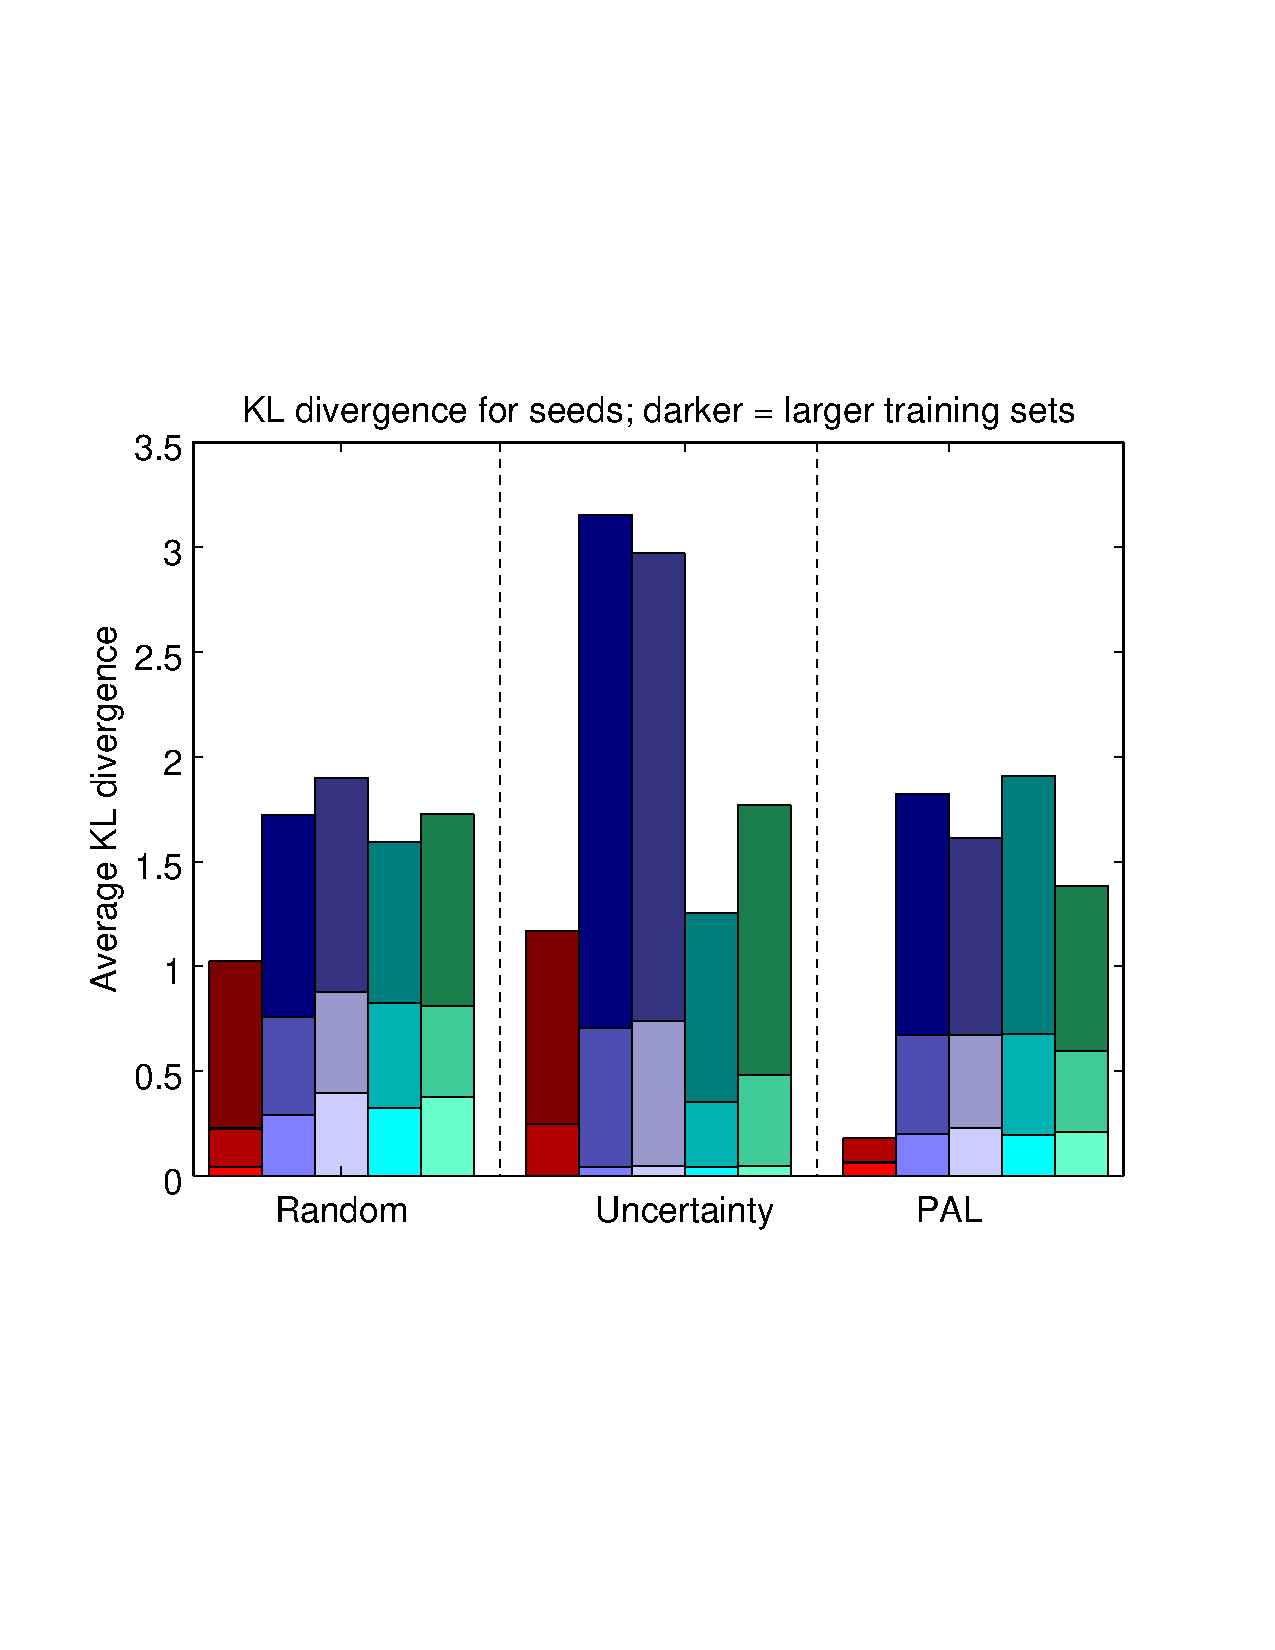
\includegraphics[trim = 1.5cm 6cm 2.5cm 6cm, clip = true, width = 0.48\textwidth]{klDivseeds}
	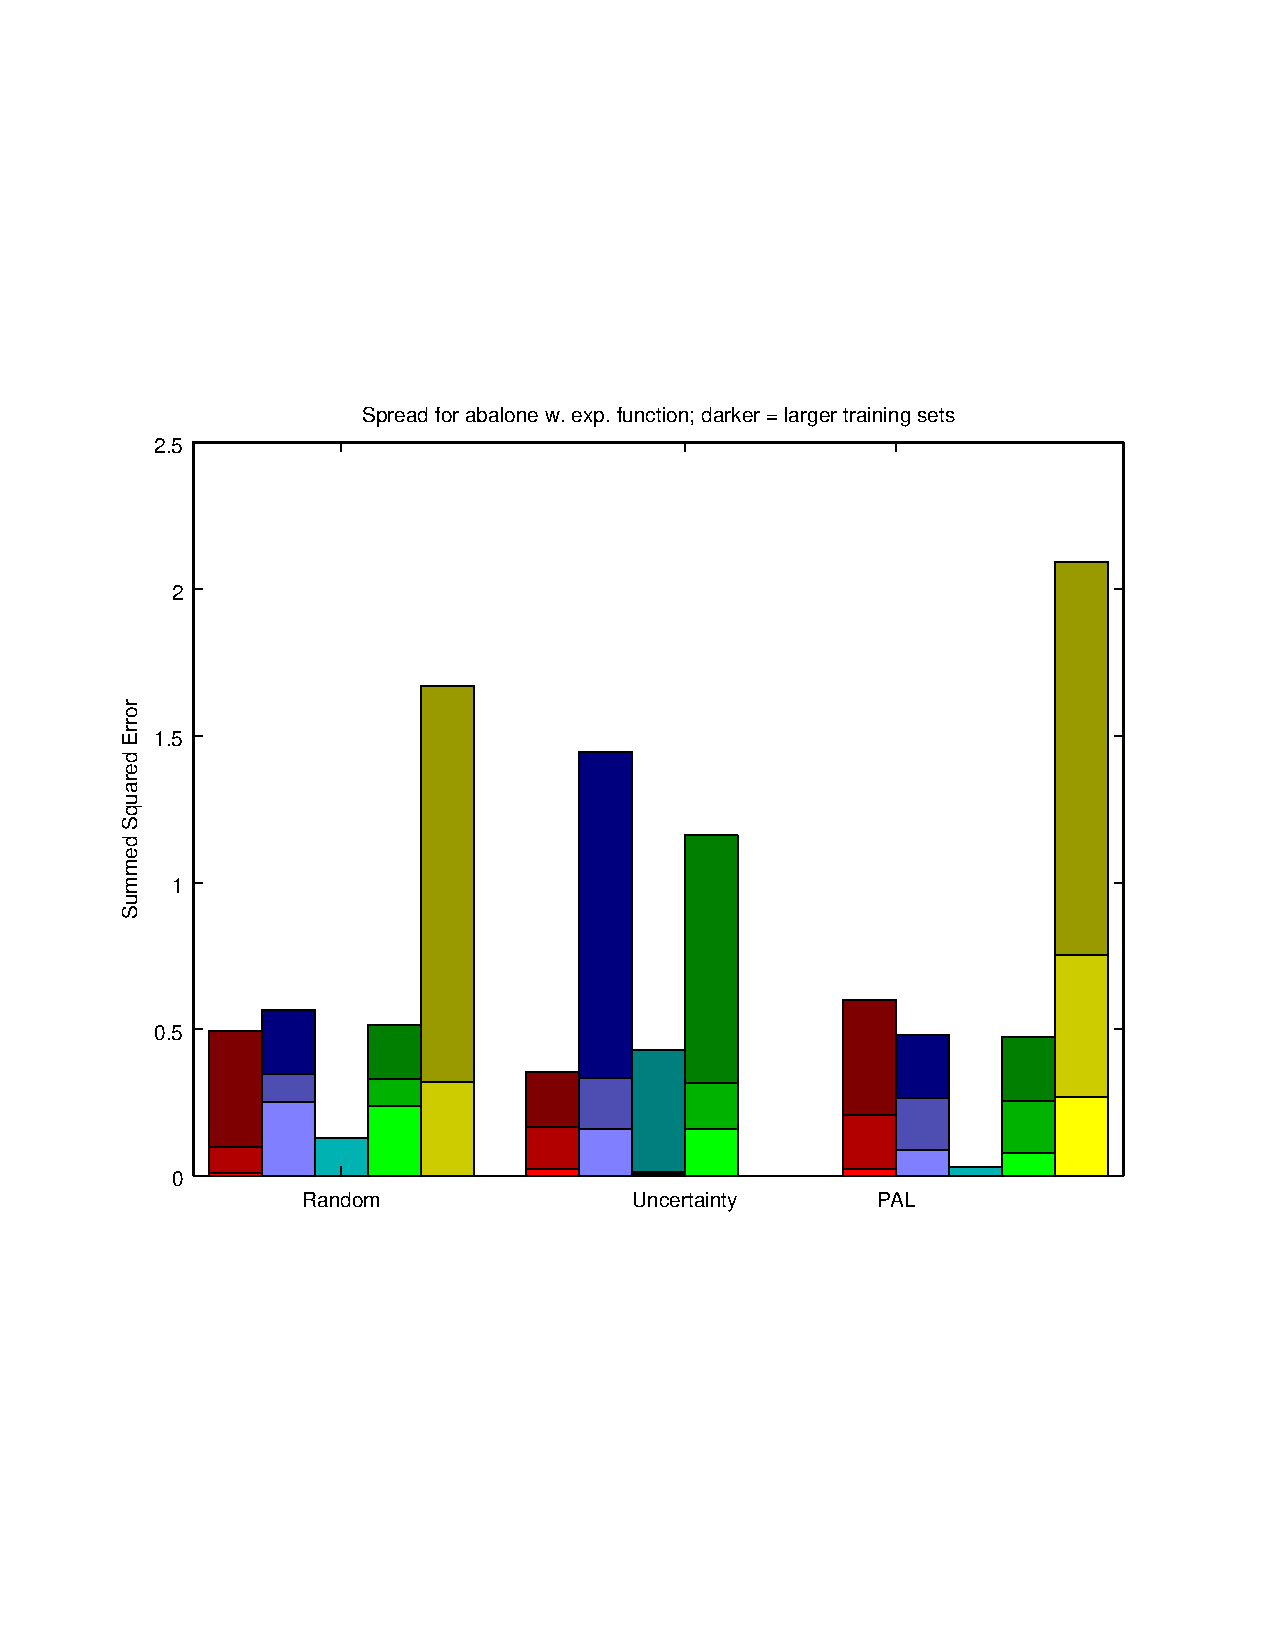
\includegraphics[trim = 1.5cm 6cm 2.5cm 6cm, clip = true, width = 0.48\textwidth]{klDivabalone}
	\caption{Kullback-Leibler divergence }
	\label{fig:klDiv}
\end{figure}

\begin{figure}[h]
	\centering
	\includegraphics[width = 0.8\textwidth]{base}
	\caption{Kullback-Leibler divergence}
	\label{fig:timeHist}
\end{figure}

\subsection{Computation Time}

TODO: Parameters, Results, Discussion etc.

TODO: abstract, introduction, conclusion

TODO: diagrams for KDE, datasets, PAL illustration
